\documentclass[twoside]{book}

% Packages required by doxygen
\usepackage{fixltx2e}
\usepackage{calc}
\usepackage{doxygen}
\usepackage[export]{adjustbox} % also loads graphicx
\usepackage{graphicx}
\usepackage[utf8]{inputenc}
\usepackage{makeidx}
\usepackage{multicol}
\usepackage{multirow}
\PassOptionsToPackage{warn}{textcomp}
\usepackage{textcomp}
\usepackage[nointegrals]{wasysym}
\usepackage[table]{xcolor}

% Font selection
\usepackage[T1]{fontenc}
\usepackage[scaled=.90]{helvet}
\usepackage{courier}
\usepackage{amssymb}
\usepackage{sectsty}
\renewcommand{\familydefault}{\sfdefault}
\allsectionsfont{%
  \fontseries{bc}\selectfont%
  \color{darkgray}%
}
\renewcommand{\DoxyLabelFont}{%
  \fontseries{bc}\selectfont%
  \color{darkgray}%
}
\newcommand{\+}{\discretionary{\mbox{\scriptsize$\hookleftarrow$}}{}{}}

% Page & text layout
\usepackage{geometry}
\geometry{%
  a4paper,%
  top=2.5cm,%
  bottom=2.5cm,%
  left=2.5cm,%
  right=2.5cm%
}
\tolerance=750
\hfuzz=15pt
\hbadness=750
\setlength{\emergencystretch}{15pt}
\setlength{\parindent}{0cm}
\setlength{\parskip}{3ex plus 2ex minus 2ex}
\makeatletter
\renewcommand{\paragraph}{%
  \@startsection{paragraph}{4}{0ex}{-1.0ex}{1.0ex}{%
    \normalfont\normalsize\bfseries\SS@parafont%
  }%
}
\renewcommand{\subparagraph}{%
  \@startsection{subparagraph}{5}{0ex}{-1.0ex}{1.0ex}{%
    \normalfont\normalsize\bfseries\SS@subparafont%
  }%
}
\makeatother

% Headers & footers
\usepackage{fancyhdr}
\pagestyle{fancyplain}
\fancyhead[LE]{\fancyplain{}{\bfseries\thepage}}
\fancyhead[CE]{\fancyplain{}{}}
\fancyhead[RE]{\fancyplain{}{\bfseries\leftmark}}
\fancyhead[LO]{\fancyplain{}{\bfseries\rightmark}}
\fancyhead[CO]{\fancyplain{}{}}
\fancyhead[RO]{\fancyplain{}{\bfseries\thepage}}
\fancyfoot[LE]{\fancyplain{}{}}
\fancyfoot[CE]{\fancyplain{}{}}
\fancyfoot[RE]{\fancyplain{}{\bfseries\scriptsize Generated by Doxygen }}
\fancyfoot[LO]{\fancyplain{}{\bfseries\scriptsize Generated by Doxygen }}
\fancyfoot[CO]{\fancyplain{}{}}
\fancyfoot[RO]{\fancyplain{}{}}
\renewcommand{\footrulewidth}{0.4pt}
\renewcommand{\chaptermark}[1]{%
  \markboth{#1}{}%
}
\renewcommand{\sectionmark}[1]{%
  \markright{\thesection\ #1}%
}

% Indices & bibliography
\usepackage{natbib}
\usepackage[titles]{tocloft}
\setcounter{tocdepth}{3}
\setcounter{secnumdepth}{5}
\makeindex

% Hyperlinks (required, but should be loaded last)
\usepackage{ifpdf}
\ifpdf
  \usepackage[pdftex,pagebackref=true]{hyperref}
\else
  \usepackage[ps2pdf,pagebackref=true]{hyperref}
\fi
\hypersetup{%
  colorlinks=true,%
  linkcolor=blue,%
  citecolor=blue,%
  unicode%
}

% Custom commands
\newcommand{\clearemptydoublepage}{%
  \newpage{\pagestyle{empty}\cleardoublepage}%
}

\usepackage{caption}
\captionsetup{labelsep=space,justification=centering,font={bf},singlelinecheck=off,skip=4pt,position=top}

%===== C O N T E N T S =====

\begin{document}

% Titlepage & ToC
\hypersetup{pageanchor=false,
             bookmarksnumbered=true,
             pdfencoding=unicode
            }
\pagenumbering{roman}
\begin{titlepage}
\vspace*{7cm}
\begin{center}%
{\Large Electric Tiger D\+AQ \\[1ex]\large 1.\+0.\+0 }\\
\vspace*{1cm}
{\large Generated by Doxygen 1.8.11}\\
\end{center}
\end{titlepage}
\clearemptydoublepage
\tableofcontents
\clearemptydoublepage
\pagenumbering{arabic}
\hypersetup{pageanchor=true}

%--- Begin generated contents ---
\chapter{Tiger-\/\+Acquire ( The D\+AQ for the Electric Tiger Experiment )}
\label{md__home_bephillips2_Qt-Projects_Electric_Tiger_DAQ_README}
\hypertarget{md__home_bephillips2_Qt-Projects_Electric_Tiger_DAQ_README}{}
This is the data acquisition system for the Electric Tiger experiment.

\section*{Dependencies}

\subsubsection*{Base}

You will need a copy of Qt5 ( version 5.\+7 or greater ) along with \href{https://doc.qt.io/qt-5/qtcharts-index.html}{\tt Qt-\/\+Charts} with should be included in the most recent versions of Qt.

You will also need the Alazartech-\/\+A\+T\+S9452 library to interface with the A\+T\+S9462 digitizer and J\+A\+S\+PL to handle signal processing.


\begin{DoxyItemize}
\item \href{http://doc.qt.io/qt-5/build-sources.html}{\tt Qt $>$= 5.\+7}
\item \href{https://github.com/bejphil/JASPL}{\tt J\+A\+S\+PL}
\item \href{https://github.com/bejphil/Alazartech-ATS9462}{\tt Alazartech-\/\+A\+T\+S9462}
\end{DoxyItemize}

\subsubsection*{Compilier requirements}


\begin{DoxyItemize}
\item \mbox{[}Opem\+MP Support (e.\+g. G\+CC)\mbox{]}
\item \mbox{[}C++11 Compliant (e.\+g. G\+CC $>$= 4.\+8.\+2\mbox{]}
\end{DoxyItemize}

\subsection*{Authors}


\begin{DoxyItemize}
\item {\bfseries Benjamin J Phillips} -\/ {\itshape As part of the Axion Dark Matter Experiment ( A\+D\+MX )} 
\end{DoxyItemize}
\chapter{Hierarchical Index}
\section{Class Hierarchy}
This inheritance list is sorted roughly, but not completely, alphabetically\+:\begin{DoxyCompactList}
\item \contentsline{section}{Config\+Processor}{\pageref{class_config_processor}}{}
\item \contentsline{section}{data\+\_\+triple$<$ T $>$}{\pageref{structdata__triple}}{}
\item exception\begin{DoxyCompactList}
\item \contentsline{section}{etig\+:\+:daq\+\_\+failure}{\pageref{classetig_1_1daq__failure}}{}
\item \contentsline{section}{mode\+\_\+track\+\_\+failure}{\pageref{classmode__track__failure}}{}
\end{DoxyCompactList}
\item \contentsline{section}{Experiment\+Parameters}{\pageref{class_experiment_parameters}}{}
\item \contentsline{section}{Flat\+File\+Saver}{\pageref{class_flat_file_saver}}{}
\item \contentsline{section}{Mode\+Track}{\pageref{class_mode_track}}{}
\item \contentsline{section}{Mode\+Traits}{\pageref{class_mode_traits}}{}
\item \contentsline{section}{Plain\+Data\+Param$<$ T $>$}{\pageref{struct_plain_data_param}}{}
\item Q\+Chart\+View\begin{DoxyCompactList}
\item \contentsline{section}{Instrument\+View}{\pageref{class_instrument_view}}{}
\item \contentsline{section}{Spectrum\+Analyzer}{\pageref{class_spectrum_analyzer}}{}
\end{DoxyCompactList}
\item Q\+Dock\+Widget\begin{DoxyCompactList}
\item \contentsline{section}{Combo\+Status\+Panel}{\pageref{class_combo_status_panel}}{}
\item \contentsline{section}{Frequency\+Controls}{\pageref{class_frequency_controls}}{}
\item \contentsline{section}{Power\+Controls}{\pageref{class_power_controls}}{}
\end{DoxyCompactList}
\item Q\+Main\+Window\begin{DoxyCompactList}
\item \contentsline{section}{Main\+Window}{\pageref{class_main_window}}{}
\end{DoxyCompactList}
\item Q\+Menu\begin{DoxyCompactList}
\item \contentsline{section}{Right\+Click\+Menu}{\pageref{class_right_click_menu}}{}
\end{DoxyCompactList}
\item Q\+Object\begin{DoxyCompactList}
\item \contentsline{section}{Abstract\+Intermitten\+Socket}{\pageref{class_abstract_intermitten_socket}}{}
\begin{DoxyCompactList}
\item \contentsline{section}{Stepper\+Motor}{\pageref{class_stepper_motor}}{}
\end{DoxyCompactList}
\item \contentsline{section}{Abstract\+Socket\+Communicator}{\pageref{class_abstract_socket_communicator}}{}
\begin{DoxyCompactList}
\item \contentsline{section}{Arduino}{\pageref{class_arduino}}{}
\item \contentsline{section}{Network\+Analyzer}{\pageref{class_network_analyzer}}{}
\item \contentsline{section}{Signal\+Generator}{\pageref{class_signal_generator}}{}
\item \contentsline{section}{Switch}{\pageref{class_switch}}{}
\end{DoxyCompactList}
\item \contentsline{section}{etig\+:\+:Program\+Core}{\pageref{classetig_1_1_program_core}}{}
\begin{DoxyCompactList}
\item \contentsline{section}{etig\+:\+:Program\+Frame}{\pageref{classetig_1_1_program_frame}}{}
\begin{DoxyCompactList}
\item \contentsline{section}{etig\+:\+:Program}{\pageref{classetig_1_1_program}}{}
\end{DoxyCompactList}
\end{DoxyCompactList}
\item \contentsline{section}{Q\+Socket\+Comm}{\pageref{class_q_socket_comm}}{}
\item \contentsline{section}{Q\+Socket\+Intermitten}{\pageref{class_q_socket_intermitten}}{}
\end{DoxyCompactList}
\item \contentsline{section}{etig\+:\+:Rebin$<$ T $>$}{\pageref{structetig_1_1_rebin}}{}
\item \contentsline{section}{etig\+:\+:Rebin$<$ float $>$}{\pageref{structetig_1_1_rebin}}{}
\item \contentsline{section}{Retrieve\+Val}{\pageref{struct_retrieve_val}}{}
\item \contentsline{section}{Socket\+Comm}{\pageref{class_socket_comm}}{}
\item \contentsline{section}{T\+C\+P\+Socket\+Param}{\pageref{struct_t_c_p_socket_param}}{}
\item \contentsline{section}{Test\+Config\+Processor}{\pageref{class_test_config_processor}}{}
\item \contentsline{section}{etig\+:\+:test\+:\+:Test\+Instrument\+View}{\pageref{classetig_1_1test_1_1_test_instrument_view}}{}
\item \contentsline{section}{etig\+:\+:test\+:\+:Test\+Panels}{\pageref{classetig_1_1test_1_1_test_panels}}{}
\item \contentsline{section}{etig\+:\+:test\+:\+:Test\+Spectrum\+Analyzer}{\pageref{classetig_1_1test_1_1_test_spectrum_analyzer}}{}
\item \contentsline{section}{etig\+:\+:test\+:\+:Volts\+Sqr\+Tod\+Bm}{\pageref{structetig_1_1test_1_1_volts_sqr_tod_bm}}{}
\end{DoxyCompactList}

\chapter{Class Index}
\section{Class List}
Here are the classes, structs, unions and interfaces with brief descriptions\+:\begin{DoxyCompactList}
\item\contentsline{section}{\hyperlink{class_abstract_intermitten_socket}{Abstract\+Intermitten\+Socket} }{\pageref{class_abstract_intermitten_socket}}{}
\item\contentsline{section}{\hyperlink{class_abstract_socket_communicator}{Abstract\+Socket\+Communicator} }{\pageref{class_abstract_socket_communicator}}{}
\item\contentsline{section}{\hyperlink{class_arduino}{Arduino} \\*Object to send and receive commands from an \hyperlink{class_arduino}{Arduino} Uno (R3) }{\pageref{class_arduino}}{}
\item\contentsline{section}{\hyperlink{class_combo_status_panel}{Combo\+Status\+Panel} }{\pageref{class_combo_status_panel}}{}
\item\contentsline{section}{\hyperlink{class_config_processor}{Config\+Processor} }{\pageref{class_config_processor}}{}
\item\contentsline{section}{\hyperlink{classetig_1_1daq__failure}{etig\+::daq\+\_\+failure} }{\pageref{classetig_1_1daq__failure}}{}
\item\contentsline{section}{\hyperlink{structdata__triple}{data\+\_\+triple$<$ T $>$} }{\pageref{structdata__triple}}{}
\item\contentsline{section}{\hyperlink{class_experiment_parameters}{Experiment\+Parameters} }{\pageref{class_experiment_parameters}}{}
\item\contentsline{section}{\hyperlink{class_flat_file_saver}{Flat\+File\+Saver} }{\pageref{class_flat_file_saver}}{}
\item\contentsline{section}{\hyperlink{class_frequency_controls}{Frequency\+Controls} }{\pageref{class_frequency_controls}}{}
\item\contentsline{section}{\hyperlink{class_instrument_view}{Instrument\+View} }{\pageref{class_instrument_view}}{}
\item\contentsline{section}{\hyperlink{class_main_window}{Main\+Window} }{\pageref{class_main_window}}{}
\item\contentsline{section}{\hyperlink{classmode__track__failure}{mode\+\_\+track\+\_\+failure} }{\pageref{classmode__track__failure}}{}
\item\contentsline{section}{\hyperlink{class_mode_track}{Mode\+Track} \\*Base Class for mode tracking algorithims; designed to be wrapped with Swig and called from Python module }{\pageref{class_mode_track}}{}
\item\contentsline{section}{\hyperlink{class_mode_traits}{Mode\+Traits} }{\pageref{class_mode_traits}}{}
\item\contentsline{section}{\hyperlink{class_network_analyzer}{Network\+Analyzer} \\*Object to communicate with the H\+P8757 C Network Analyzer }{\pageref{class_network_analyzer}}{}
\item\contentsline{section}{\hyperlink{struct_plain_data_param}{Plain\+Data\+Param$<$ T $>$} }{\pageref{struct_plain_data_param}}{}
\item\contentsline{section}{\hyperlink{class_power_controls}{Power\+Controls} }{\pageref{class_power_controls}}{}
\item\contentsline{section}{\hyperlink{classetig_1_1_program}{etig\+::\+Program} }{\pageref{classetig_1_1_program}}{}
\item\contentsline{section}{\hyperlink{classetig_1_1_program_core}{etig\+::\+Program\+Core} }{\pageref{classetig_1_1_program_core}}{}
\item\contentsline{section}{\hyperlink{classetig_1_1_program_frame}{etig\+::\+Program\+Frame} }{\pageref{classetig_1_1_program_frame}}{}
\item\contentsline{section}{\hyperlink{class_q_socket_comm}{Q\+Socket\+Comm} }{\pageref{class_q_socket_comm}}{}
\item\contentsline{section}{\hyperlink{class_q_socket_intermitten}{Q\+Socket\+Intermitten} }{\pageref{class_q_socket_intermitten}}{}
\item\contentsline{section}{\hyperlink{structetig_1_1_rebin}{etig\+::\+Rebin$<$ T $>$} }{\pageref{structetig_1_1_rebin}}{}
\item\contentsline{section}{\hyperlink{struct_retrieve_val}{Retrieve\+Val} }{\pageref{struct_retrieve_val}}{}
\item\contentsline{section}{\hyperlink{class_right_click_menu}{Right\+Click\+Menu} }{\pageref{class_right_click_menu}}{}
\item\contentsline{section}{\hyperlink{class_signal_generator}{Signal\+Generator} }{\pageref{class_signal_generator}}{}
\item\contentsline{section}{\hyperlink{class_socket_comm}{Socket\+Comm} }{\pageref{class_socket_comm}}{}
\item\contentsline{section}{\hyperlink{class_spectrum_analyzer}{Spectrum\+Analyzer} }{\pageref{class_spectrum_analyzer}}{}
\item\contentsline{section}{\hyperlink{class_stepper_motor}{Stepper\+Motor} \\*Object to sends commands to an Applied Motion products stepper motor }{\pageref{class_stepper_motor}}{}
\item\contentsline{section}{\hyperlink{class_switch}{Switch} }{\pageref{class_switch}}{}
\item\contentsline{section}{\hyperlink{struct_t_c_p_socket_param}{T\+C\+P\+Socket\+Param} }{\pageref{struct_t_c_p_socket_param}}{}
\item\contentsline{section}{\hyperlink{class_test_config_processor}{Test\+Config\+Processor} }{\pageref{class_test_config_processor}}{}
\item\contentsline{section}{\hyperlink{classetig_1_1test_1_1_test_instrument_view}{etig\+::test\+::\+Test\+Instrument\+View} }{\pageref{classetig_1_1test_1_1_test_instrument_view}}{}
\item\contentsline{section}{\hyperlink{classetig_1_1test_1_1_test_panels}{etig\+::test\+::\+Test\+Panels} }{\pageref{classetig_1_1test_1_1_test_panels}}{}
\item\contentsline{section}{\hyperlink{classetig_1_1test_1_1_test_spectrum_analyzer}{etig\+::test\+::\+Test\+Spectrum\+Analyzer} }{\pageref{classetig_1_1test_1_1_test_spectrum_analyzer}}{}
\item\contentsline{section}{\hyperlink{structetig_1_1test_1_1_volts_sqr_tod_bm}{etig\+::test\+::\+Volts\+Sqr\+Tod\+Bm} }{\pageref{structetig_1_1test_1_1_volts_sqr_tod_bm}}{}
\end{DoxyCompactList}

\chapter{Class Documentation}
\hypertarget{class_abstract_intermitten_socket}{}\section{Abstract\+Intermitten\+Socket Class Reference}
\label{class_abstract_intermitten_socket}\index{Abstract\+Intermitten\+Socket@{Abstract\+Intermitten\+Socket}}


Inheritance diagram for Abstract\+Intermitten\+Socket\+:\nopagebreak
\begin{figure}[H]
\begin{center}
\leavevmode
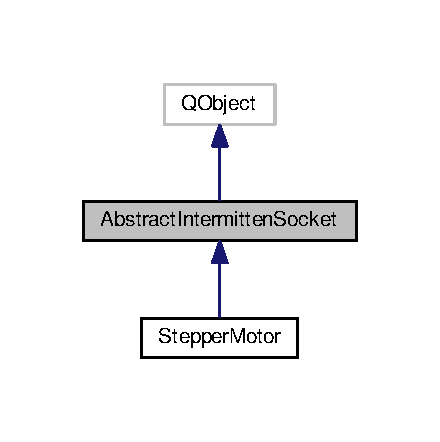
\includegraphics[width=211pt]{class_abstract_intermitten_socket__inherit__graph}
\end{center}
\end{figure}


Collaboration diagram for Abstract\+Intermitten\+Socket\+:\nopagebreak
\begin{figure}[H]
\begin{center}
\leavevmode
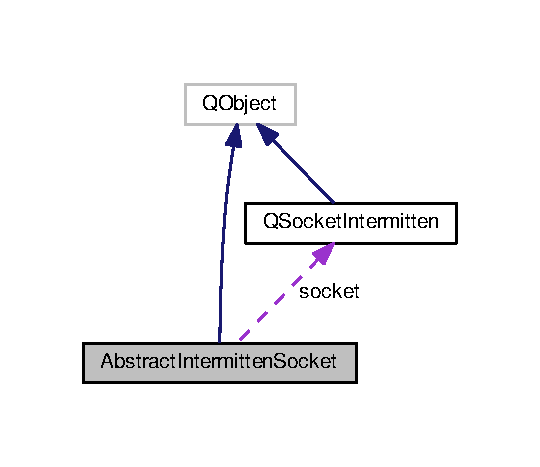
\includegraphics[width=259pt]{class_abstract_intermitten_socket__coll__graph}
\end{center}
\end{figure}
\subsection*{Public Member Functions}
\begin{DoxyCompactItemize}
\item 
{\bfseries Abstract\+Intermitten\+Socket} (std\+::string ip\+\_\+addr, uint port\+\_\+number, Q\+Object $\ast$parent=0)\hypertarget{class_abstract_intermitten_socket_a6da643b4105a119af6e855bd2885656a}{}\label{class_abstract_intermitten_socket_a6da643b4105a119af6e855bd2885656a}

\item 
{\bfseries Abstract\+Intermitten\+Socket} (const \hyperlink{struct_t_c_p_socket_param}{T\+C\+P\+Socket\+Param} socket\+\_\+param, Q\+Object $\ast$parent=0)\hypertarget{class_abstract_intermitten_socket_ab16868d5b1dd0349c64d9ec5eae8707b}{}\label{class_abstract_intermitten_socket_ab16868d5b1dd0349c64d9ec5eae8707b}

\item 
\hyperlink{class_abstract_intermitten_socket}{Abstract\+Intermitten\+Socket} \& {\bfseries operator=} (const \hyperlink{class_abstract_intermitten_socket}{Abstract\+Intermitten\+Socket} \&)=delete\hypertarget{class_abstract_intermitten_socket_a2be6aa5fe81ced7c9f2ad7b32978d990}{}\label{class_abstract_intermitten_socket_a2be6aa5fe81ced7c9f2ad7b32978d990}

\end{DoxyCompactItemize}
\subsection*{Protected Attributes}
\begin{DoxyCompactItemize}
\item 
\hyperlink{class_q_socket_intermitten}{Q\+Socket\+Intermitten} $\ast$ {\bfseries socket}\hypertarget{class_abstract_intermitten_socket_af086bed84ba4bc6d5137d3c9486f0077}{}\label{class_abstract_intermitten_socket_af086bed84ba4bc6d5137d3c9486f0077}

\end{DoxyCompactItemize}


The documentation for this class was generated from the following files\+:\begin{DoxyCompactItemize}
\item 
/home/bephillips2/\+Qt-\/\+Projects/\+Electric\+\_\+\+Tiger\+\_\+\+D\+A\+Q/\+Socket\+Communicators/\+Abstract\+Socket\+Communicator/abstractintermittensocket.\+h\item 
/home/bephillips2/\+Qt-\/\+Projects/\+Electric\+\_\+\+Tiger\+\_\+\+D\+A\+Q/\+Socket\+Communicators/\+Abstract\+Socket\+Communicator/abstractintermittensocket.\+cpp\end{DoxyCompactItemize}

\hypertarget{class_abstract_socket_communicator}{}\section{Abstract\+Socket\+Communicator Class Reference}
\label{class_abstract_socket_communicator}\index{Abstract\+Socket\+Communicator@{Abstract\+Socket\+Communicator}}


Inheritance diagram for Abstract\+Socket\+Communicator\+:\nopagebreak
\begin{figure}[H]
\begin{center}
\leavevmode
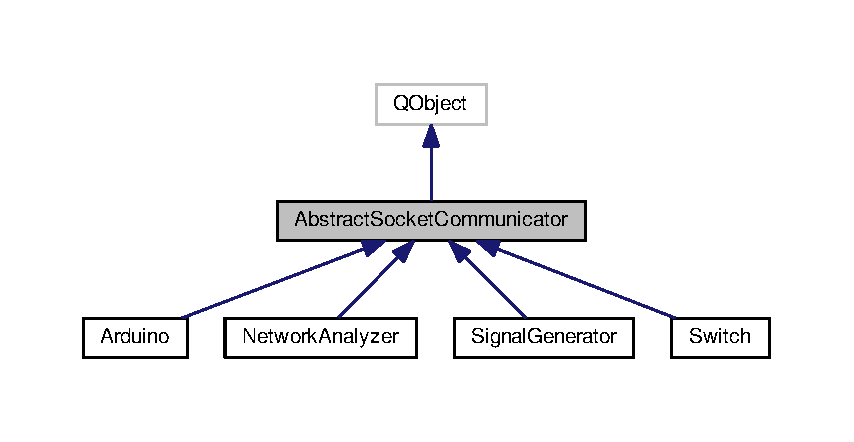
\includegraphics[width=350pt]{class_abstract_socket_communicator__inherit__graph}
\end{center}
\end{figure}


Collaboration diagram for Abstract\+Socket\+Communicator\+:\nopagebreak
\begin{figure}[H]
\begin{center}
\leavevmode
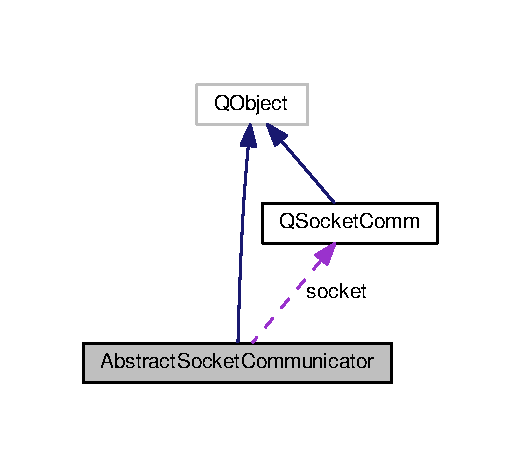
\includegraphics[width=250pt]{class_abstract_socket_communicator__coll__graph}
\end{center}
\end{figure}
\subsection*{Public Member Functions}
\begin{DoxyCompactItemize}
\item 
{\bfseries Abstract\+Socket\+Communicator} (std\+::string ip\+\_\+addr, uint port\+\_\+number, Q\+Object $\ast$parent=0)\hypertarget{class_abstract_socket_communicator_a421d86ea7de8b9f2e726e4c1a8a03a42}{}\label{class_abstract_socket_communicator_a421d86ea7de8b9f2e726e4c1a8a03a42}

\item 
{\bfseries Abstract\+Socket\+Communicator} (const \hyperlink{struct_t_c_p_socket_param}{T\+C\+P\+Socket\+Param} socket\+\_\+param, Q\+Object $\ast$parent=0)\hypertarget{class_abstract_socket_communicator_a84fed194f0cb2cca744be18d741d6129}{}\label{class_abstract_socket_communicator_a84fed194f0cb2cca744be18d741d6129}

\item 
\hyperlink{class_abstract_socket_communicator}{Abstract\+Socket\+Communicator} \& {\bfseries operator=} (const \hyperlink{class_abstract_socket_communicator}{Abstract\+Socket\+Communicator} \&)=delete\hypertarget{class_abstract_socket_communicator_a7ee57a3af5927ac08f515055dbcdc829}{}\label{class_abstract_socket_communicator_a7ee57a3af5927ac08f515055dbcdc829}

\end{DoxyCompactItemize}
\subsection*{Protected Attributes}
\begin{DoxyCompactItemize}
\item 
\hyperlink{class_q_socket_comm}{Q\+Socket\+Comm} $\ast$ {\bfseries socket}\hypertarget{class_abstract_socket_communicator_a7e69037572c26cf596bd117490f9d6c1}{}\label{class_abstract_socket_communicator_a7e69037572c26cf596bd117490f9d6c1}

\end{DoxyCompactItemize}


The documentation for this class was generated from the following files\+:\begin{DoxyCompactItemize}
\item 
/home/bephillips2/\+Qt-\/\+Projects/\+Electric\+\_\+\+Tiger\+\_\+\+D\+A\+Q/\+Socket\+Communicators/\+Abstract\+Socket\+Communicator/abstractsocketcommunictor.\+h\item 
/home/bephillips2/\+Qt-\/\+Projects/\+Electric\+\_\+\+Tiger\+\_\+\+D\+A\+Q/\+Socket\+Communicators/\+Abstract\+Socket\+Communicator/abstractsocketcommunictor.\+cpp\end{DoxyCompactItemize}

\hypertarget{class_arduino}{}\section{Arduino Class Reference}
\label{class_arduino}\index{Arduino@{Arduino}}


Object to send and receive commands from an \hyperlink{class_arduino}{Arduino} Uno (R3)  




{\ttfamily \#include $<$arduino.\+h$>$}



Inheritance diagram for Arduino\+:\nopagebreak
\begin{figure}[H]
\begin{center}
\leavevmode
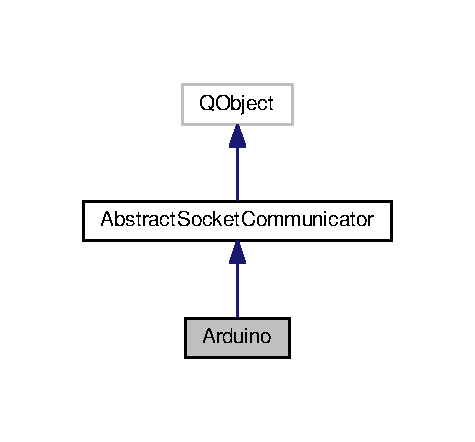
\includegraphics[width=228pt]{class_arduino__inherit__graph}
\end{center}
\end{figure}


Collaboration diagram for Arduino\+:\nopagebreak
\begin{figure}[H]
\begin{center}
\leavevmode
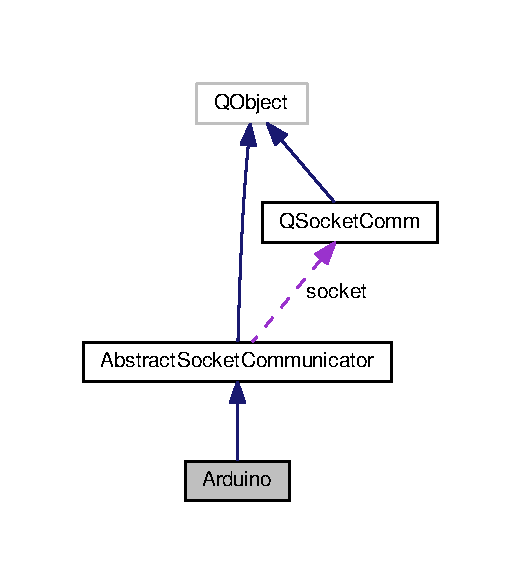
\includegraphics[width=250pt]{class_arduino__coll__graph}
\end{center}
\end{figure}
\subsection*{Public Member Functions}
\begin{DoxyCompactItemize}
\item 
{\bfseries Arduino} (std\+::string ip\+\_\+addr, uint port\+\_\+number, Q\+Object $\ast$parent=0)\hypertarget{class_arduino_a89116271522c40d0e248a6958e27e408}{}\label{class_arduino_a89116271522c40d0e248a6958e27e408}

\item 
\hyperlink{class_arduino}{Arduino} \& {\bfseries operator=} (const \hyperlink{class_arduino}{Arduino} \&)=delete\hypertarget{class_arduino_a73d294f82c38557d1872cadd372c0b8b}{}\label{class_arduino_a73d294f82c38557d1872cadd372c0b8b}

\item 
double \hyperlink{class_arduino_a0ae462174c61881ccd5f78af5130eceb}{Get\+Cavity\+Length} ()
\begin{DoxyCompactList}\small\item\em Get the current cavity length from the \hyperlink{class_arduino}{Arduino}. \end{DoxyCompactList}\end{DoxyCompactItemize}
\subsection*{Additional Inherited Members}


\subsection{Detailed Description}
Object to send and receive commands from an \hyperlink{class_arduino}{Arduino} Uno (R3) 

\hyperlink{class_arduino}{Arduino} is expected to be equipped with an Ethernet Shield and string potentiometer. 

\subsection{Member Function Documentation}
\index{Arduino@{Arduino}!Get\+Cavity\+Length@{Get\+Cavity\+Length}}
\index{Get\+Cavity\+Length@{Get\+Cavity\+Length}!Arduino@{Arduino}}
\subsubsection[{\texorpdfstring{Get\+Cavity\+Length()}{GetCavityLength()}}]{\setlength{\rightskip}{0pt plus 5cm}double Arduino\+::\+Get\+Cavity\+Length (
\begin{DoxyParamCaption}
{}
\end{DoxyParamCaption}
)}\hypertarget{class_arduino_a0ae462174c61881ccd5f78af5130eceb}{}\label{class_arduino_a0ae462174c61881ccd5f78af5130eceb}


Get the current cavity length from the \hyperlink{class_arduino}{Arduino}. 

This function will poll the \hyperlink{class_arduino}{Arduino} until a non-\/empty string is returned, guaranteeing that the return value will be valid.

Note that this does not elminate the problem of getting \textquotesingle{}doubled\textquotesingle{} responses, e.\+g. \char`\"{}7.\+5\textbackslash{}r\textbackslash{}n7.\+5\char`\"{}

\begin{DoxyReturn}{Returns}
Current length of the cavity, in inches 
\end{DoxyReturn}


The documentation for this class was generated from the following files\+:\begin{DoxyCompactItemize}
\item 
/home/bephillips2/\+Qt-\/\+Projects/\+Electric\+\_\+\+Tiger\+\_\+\+D\+A\+Q/\+Socket\+Communicators/\+Arduino/arduino.\+h\item 
/home/bephillips2/\+Qt-\/\+Projects/\+Electric\+\_\+\+Tiger\+\_\+\+D\+A\+Q/\+Socket\+Communicators/\+Arduino/arduino.\+cpp\end{DoxyCompactItemize}

\hypertarget{class_combo_status_panel}{}\section{Combo\+Status\+Panel Class Reference}
\label{class_combo_status_panel}\index{Combo\+Status\+Panel@{Combo\+Status\+Panel}}


Inheritance diagram for Combo\+Status\+Panel\+:\nopagebreak
\begin{figure}[H]
\begin{center}
\leavevmode
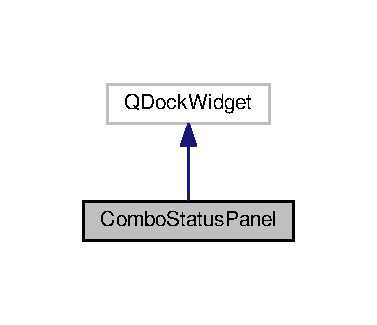
\includegraphics[width=181pt]{class_combo_status_panel__inherit__graph}
\end{center}
\end{figure}


Collaboration diagram for Combo\+Status\+Panel\+:\nopagebreak
\begin{figure}[H]
\begin{center}
\leavevmode
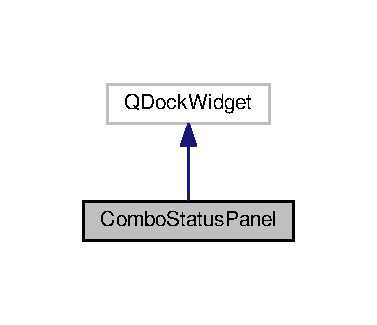
\includegraphics[width=181pt]{class_combo_status_panel__coll__graph}
\end{center}
\end{figure}
\subsection*{Public Slots}
\begin{DoxyCompactItemize}
\item 
void {\bfseries Set\+Transmission} ()\hypertarget{class_combo_status_panel_a926b00ce9496c55077ac5719dcd7bdeb}{}\label{class_combo_status_panel_a926b00ce9496c55077ac5719dcd7bdeb}

\item 
void {\bfseries Set\+Reflection} ()\hypertarget{class_combo_status_panel_a8e949a09cf250c66c645d982eac012ef}{}\label{class_combo_status_panel_a8e949a09cf250c66c645d982eac012ef}

\item 
void {\bfseries Set\+Digitizer} ()\hypertarget{class_combo_status_panel_ad3c4a3aab45aa2663806805e7330e4be}{}\label{class_combo_status_panel_ad3c4a3aab45aa2663806805e7330e4be}

\item 
void {\bfseries Set\+Network\+Analyzer} ()\hypertarget{class_combo_status_panel_a276208d722c7173d801464bb9cd39f17}{}\label{class_combo_status_panel_a276208d722c7173d801464bb9cd39f17}

\item 
void {\bfseries Set\+Iteration\+Number} (uint iteration)\hypertarget{class_combo_status_panel_acd114441ad2cf073f9bd734369430a5b}{}\label{class_combo_status_panel_acd114441ad2cf073f9bd734369430a5b}

\item 
void {\bfseries Set\+Cavity\+Length} (double current\+\_\+length)\hypertarget{class_combo_status_panel_aa1894532aba11f13402781d260dcb82e}{}\label{class_combo_status_panel_aa1894532aba11f13402781d260dcb82e}

\item 
void {\bfseries Set\+L\+O\+Frequency} (double lo\+\_\+frequency)\hypertarget{class_combo_status_panel_a42fc2fc8fc9c24cdcb569ee12a70afb5}{}\label{class_combo_status_panel_a42fc2fc8fc9c24cdcb569ee12a70afb5}

\end{DoxyCompactItemize}
\subsection*{Public Member Functions}
\begin{DoxyCompactItemize}
\item 
{\bfseries Combo\+Status\+Panel} (Q\+Widget $\ast$parent=0)\hypertarget{class_combo_status_panel_affde893188d5ba0ea12133682543fddc}{}\label{class_combo_status_panel_affde893188d5ba0ea12133682543fddc}

\end{DoxyCompactItemize}


The documentation for this class was generated from the following files\+:\begin{DoxyCompactItemize}
\item 
/home/bephillips2/\+Qt-\/\+Projects/\+Electric\+\_\+\+Tiger\+\_\+\+D\+A\+Q/\+Panels/\+Status\+Combo/combostatuspanel.\+h\item 
/home/bephillips2/\+Qt-\/\+Projects/\+Electric\+\_\+\+Tiger\+\_\+\+D\+A\+Q/\+Panels/\+Status\+Combo/combostatuspanel.\+cpp\end{DoxyCompactItemize}

\hypertarget{class_config_processor}{}\section{Config\+Processor Class Reference}
\label{class_config_processor}\index{Config\+Processor@{Config\+Processor}}
\subsection*{Public Member Functions}
\begin{DoxyCompactItemize}
\item 
{\bfseries Config\+Processor} (std\+::string file\+\_\+path)\hypertarget{class_config_processor_a28b19765419c2b6ddb1b3327b711f4e7}{}\label{class_config_processor_a28b19765419c2b6ddb1b3327b711f4e7}

\item 
{\footnotesize template$<$typename T $>$ }\\T {\bfseries Get\+Value} (std\+::string param\+\_\+name)\hypertarget{class_config_processor_a511cd925379b98cc4fd85d320bdb490d}{}\label{class_config_processor_a511cd925379b98cc4fd85d320bdb490d}

\end{DoxyCompactItemize}
\subsection*{Public Attributes}
\begin{DoxyCompactItemize}
\item 
std\+::vector$<$ \hyperlink{struct_plain_data_param}{Plain\+Data\+Param}$<$ double $>$ $>$ {\bfseries data\+\_\+list}\hypertarget{class_config_processor_a28ccb85933245a036982ab22a3138b17}{}\label{class_config_processor_a28ccb85933245a036982ab22a3138b17}

\item 
std\+::vector$<$ \hyperlink{struct_plain_data_param}{Plain\+Data\+Param}$<$ std\+::string $>$ $>$ {\bfseries string\+\_\+list}\hypertarget{class_config_processor_a9401084ab2e2cd556eb1c3844eefd273}{}\label{class_config_processor_a9401084ab2e2cd556eb1c3844eefd273}

\item 
std\+::vector$<$ \hyperlink{struct_t_c_p_socket_param}{T\+C\+P\+Socket\+Param} $>$ {\bfseries socket\+\_\+info\+\_\+list}\hypertarget{class_config_processor_a7f9bacfd051f7f50440f1325c96a99e6}{}\label{class_config_processor_a7f9bacfd051f7f50440f1325c96a99e6}

\end{DoxyCompactItemize}


The documentation for this class was generated from the following files\+:\begin{DoxyCompactItemize}
\item 
/home/bephillips2/\+Qt-\/\+Projects/\+Electric\+\_\+\+Tiger\+\_\+\+D\+A\+Q/\+Config\+Processor/configprocessor.\+h\item 
/home/bephillips2/\+Qt-\/\+Projects/\+Electric\+\_\+\+Tiger\+\_\+\+D\+A\+Q/\+Config\+Processor/configprocessor.\+cpp\end{DoxyCompactItemize}

\hypertarget{classetig_1_1daq__failure}{}\section{etig\+:\+:daq\+\_\+failure Class Reference}
\label{classetig_1_1daq__failure}\index{etig\+::daq\+\_\+failure@{etig\+::daq\+\_\+failure}}


Inheritance diagram for etig\+:\+:daq\+\_\+failure\+:\nopagebreak
\begin{figure}[H]
\begin{center}
\leavevmode
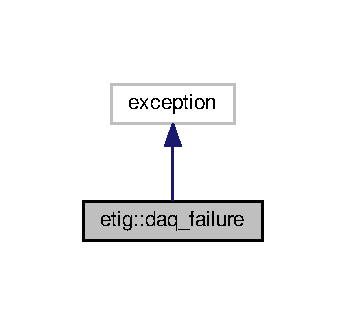
\includegraphics[width=166pt]{classetig_1_1daq__failure__inherit__graph}
\end{center}
\end{figure}


Collaboration diagram for etig\+:\+:daq\+\_\+failure\+:\nopagebreak
\begin{figure}[H]
\begin{center}
\leavevmode
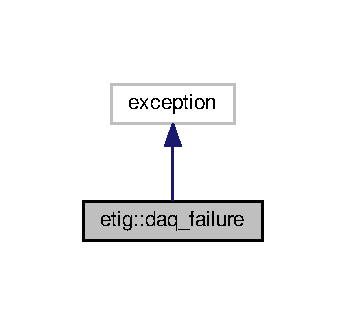
\includegraphics[width=166pt]{classetig_1_1daq__failure__coll__graph}
\end{center}
\end{figure}
\subsection*{Public Member Functions}
\begin{DoxyCompactItemize}
\item 
{\bfseries daq\+\_\+failure} (const char $\ast$message)\hypertarget{classetig_1_1daq__failure_a47f1bcf6385dc3f7107246ab0ae0259e}{}\label{classetig_1_1daq__failure_a47f1bcf6385dc3f7107246ab0ae0259e}

\item 
const char $\ast$ {\bfseries what} () const   throw ()\hypertarget{classetig_1_1daq__failure_a70e933a799676e24b6facb725f14492a}{}\label{classetig_1_1daq__failure_a70e933a799676e24b6facb725f14492a}

\end{DoxyCompactItemize}


The documentation for this class was generated from the following file\+:\begin{DoxyCompactItemize}
\item 
/home/bephillips2/\+Qt-\/\+Projects/\+Electric\+\_\+\+Tiger\+\_\+\+D\+A\+Q/\+Program/\+Program\+Core/daq\+\_\+failure.\+h\end{DoxyCompactItemize}

\hypertarget{structdata__triple}{}\section{data\+\_\+triple$<$ T $>$ Struct Template Reference}
\label{structdata__triple}\index{data\+\_\+triple$<$ T $>$@{data\+\_\+triple$<$ T $>$}}
\subsection*{Public Member Functions}
\begin{DoxyCompactItemize}
\item 
{\bfseries data\+\_\+triple} (T cav\+\_\+len, T freq, T power)\hypertarget{structdata__triple_a223be233f58eb5cb136fb0be322b4cb7}{}\label{structdata__triple_a223be233f58eb5cb136fb0be322b4cb7}

\item 
\hyperlink{structdata__triple}{data\+\_\+triple} \& {\bfseries operator=} (const \hyperlink{structdata__triple}{data\+\_\+triple} \&triple)\hypertarget{structdata__triple_a7da3f3ea534c4217ad69b110b087398c}{}\label{structdata__triple_a7da3f3ea534c4217ad69b110b087398c}

\end{DoxyCompactItemize}
\subsection*{Public Attributes}
\begin{DoxyCompactItemize}
\item 
T {\bfseries cavity\+\_\+length}\hypertarget{structdata__triple_a0c009762d01c841ed025b80a12955419}{}\label{structdata__triple_a0c009762d01c841ed025b80a12955419}

\item 
T {\bfseries frequency\+\_\+\+M\+Hz}\hypertarget{structdata__triple_a50bc0714de99feb9e3fcb1fa868d082b}{}\label{structdata__triple_a50bc0714de99feb9e3fcb1fa868d082b}

\item 
T {\bfseries power\+\_\+d\+Bm}\hypertarget{structdata__triple_a6f88f895f5d91c784ef723e87d904c14}{}\label{structdata__triple_a6f88f895f5d91c784ef723e87d904c14}

\end{DoxyCompactItemize}
\subsection*{Friends}
\begin{DoxyCompactItemize}
\item 
std\+::ostream \& {\bfseries operator$<$$<$} (std\+::ostream \&stream, const \hyperlink{structdata__triple}{data\+\_\+triple} \&triple)\hypertarget{structdata__triple_ae1f2fcec0b69760f3a5a9b97d13ec84d}{}\label{structdata__triple_ae1f2fcec0b69760f3a5a9b97d13ec84d}

\item 
std\+::ofstream \& {\bfseries operator$<$$<$} (std\+::ofstream \&stream, const \hyperlink{structdata__triple}{data\+\_\+triple} \&triple)\hypertarget{structdata__triple_a7427c6054c2f2b559c384fc92da91e77}{}\label{structdata__triple_a7427c6054c2f2b559c384fc92da91e77}

\end{DoxyCompactItemize}


The documentation for this struct was generated from the following file\+:\begin{DoxyCompactItemize}
\item 
/home/bephillips2/\+Qt-\/\+Projects/\+Electric\+\_\+\+Tiger\+\_\+\+D\+A\+Q/\+Generics/generics.\+h\end{DoxyCompactItemize}

\hypertarget{class_experiment_parameters}{}\section{Experiment\+Parameters Class Reference}
\label{class_experiment_parameters}\index{Experiment\+Parameters@{Experiment\+Parameters}}


Collaboration diagram for Experiment\+Parameters\+:\nopagebreak
\begin{figure}[H]
\begin{center}
\leavevmode
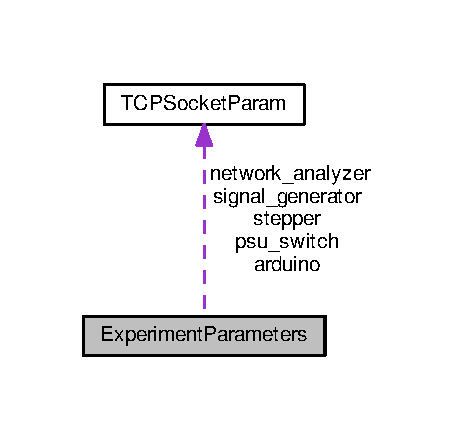
\includegraphics[width=218pt]{class_experiment_parameters__coll__graph}
\end{center}
\end{figure}
\subsection*{Public Attributes}
\begin{DoxyCompactItemize}
\item 
const std\+::string {\bfseries save\+\_\+file\+\_\+path} = \char`\"{}/home/bephillips2/workspace/Electric\+\_\+\+Tiger\+\_\+\+Control\+\_\+\+Code/data/\char`\"{}\hypertarget{class_experiment_parameters_a1cfe3a5d3b3bffce5c0b890f35d7d7ba}{}\label{class_experiment_parameters_a1cfe3a5d3b3bffce5c0b890f35d7d7ba}

\item 
const double {\bfseries length\+\_\+of\+\_\+tune} = 3.\+0\hypertarget{class_experiment_parameters_ace5c189c9e18f1137e875a6487e8fd1a}{}\label{class_experiment_parameters_ace5c189c9e18f1137e875a6487e8fd1a}

\item 
const double {\bfseries revs\+\_\+per\+\_\+iterations} = 2.\+5\hypertarget{class_experiment_parameters_ae6b8acdaee713344727231fe90cda43e}{}\label{class_experiment_parameters_ae6b8acdaee713344727231fe90cda43e}

\item 
const double {\bfseries start\+\_\+length} = 7.\+0\hypertarget{class_experiment_parameters_ae1ad144064c4d84a0356262a66f6762e}{}\label{class_experiment_parameters_ae1ad144064c4d84a0356262a66f6762e}

\item 
const double {\bfseries nwa\+\_\+span\+\_\+\+M\+Hz} = 400.\+0\hypertarget{class_experiment_parameters_ae6c893bbe23d5fa066b22a1eff53a7c0}{}\label{class_experiment_parameters_ae6c893bbe23d5fa066b22a1eff53a7c0}

\item 
const uint {\bfseries nwa\+\_\+points} = 401\hypertarget{class_experiment_parameters_a32013416c5253fb5e9a6dc1b6c18b0a1}{}\label{class_experiment_parameters_a32013416c5253fb5e9a6dc1b6c18b0a1}

\item 
const double {\bfseries nwa\+\_\+power\+\_\+d\+Bm} = -\/15.\+0\hypertarget{class_experiment_parameters_ab16b546dab57c7077152a97053a041d0}{}\label{class_experiment_parameters_ab16b546dab57c7077152a97053a041d0}

\item 
const double {\bfseries freq\+\_\+window\+\_\+\+M\+Hz} = 100.\+0\hypertarget{class_experiment_parameters_a1d495d1cadd1cb8f3221d1adc7a2e92e}{}\label{class_experiment_parameters_a1d495d1cadd1cb8f3221d1adc7a2e92e}

\item 
const double {\bfseries digitizer\+\_\+rate\+\_\+\+M\+Hz} = 50.\+0\hypertarget{class_experiment_parameters_acfd9ce58ec8a3407d76c10db7a33168e}{}\label{class_experiment_parameters_acfd9ce58ec8a3407d76c10db7a33168e}

\item 
const uint {\bfseries num\+\_\+averages} = 10000\hypertarget{class_experiment_parameters_a7434e2b3a7f7eccdc212cc55651922e2}{}\label{class_experiment_parameters_a7434e2b3a7f7eccdc212cc55651922e2}

\item 
const \hyperlink{struct_t_c_p_socket_param}{T\+C\+P\+Socket\+Param} {\bfseries psu\+\_\+switch} = \hyperlink{struct_t_c_p_socket_param}{T\+C\+P\+Socket\+Param}( \char`\"{}Switch\char`\"{}, \char`\"{}10.\+95.\+100.\+174\char`\"{}, 9221 )\hypertarget{class_experiment_parameters_ae700482ce71b3a5558ee41093913297a}{}\label{class_experiment_parameters_ae700482ce71b3a5558ee41093913297a}

\item 
const \hyperlink{struct_t_c_p_socket_param}{T\+C\+P\+Socket\+Param} {\bfseries network\+\_\+analyzer} = \hyperlink{struct_t_c_p_socket_param}{T\+C\+P\+Socket\+Param}( \char`\"{}Network\+Analyzer\char`\"{}, \char`\"{}10.\+95.\+100.\+176\char`\"{}, 1234 )\hypertarget{class_experiment_parameters_afa22bbf371056c9f48ab16fc75ae8bc7}{}\label{class_experiment_parameters_afa22bbf371056c9f48ab16fc75ae8bc7}

\item 
const \hyperlink{struct_t_c_p_socket_param}{T\+C\+P\+Socket\+Param} {\bfseries stepper} = \hyperlink{struct_t_c_p_socket_param}{T\+C\+P\+Socket\+Param}( \char`\"{}Stepper\char`\"{}, \char`\"{}10.\+95.\+100.\+177\char`\"{}, 7776 )\hypertarget{class_experiment_parameters_ae51cbbd261707bafe2cfd50cef214cb5}{}\label{class_experiment_parameters_ae51cbbd261707bafe2cfd50cef214cb5}

\item 
const \hyperlink{struct_t_c_p_socket_param}{T\+C\+P\+Socket\+Param} {\bfseries signal\+\_\+generator} = \hyperlink{struct_t_c_p_socket_param}{T\+C\+P\+Socket\+Param}( \char`\"{}Signal\+Generator\char`\"{}, \char`\"{}10.\+95.\+100.\+175\char`\"{}, 5025 )\hypertarget{class_experiment_parameters_a3433956c9a6d19db55ce7ea22c3ec731}{}\label{class_experiment_parameters_a3433956c9a6d19db55ce7ea22c3ec731}

\item 
const \hyperlink{struct_t_c_p_socket_param}{T\+C\+P\+Socket\+Param} {\bfseries arduino} = \hyperlink{struct_t_c_p_socket_param}{T\+C\+P\+Socket\+Param}( \char`\"{}Arduino\char`\"{}, \char`\"{};10.\+66.\+192.\+41\char`\"{}, 23 )\hypertarget{class_experiment_parameters_a3657583fc47ddc41cacc1954297fe8ba}{}\label{class_experiment_parameters_a3657583fc47ddc41cacc1954297fe8ba}

\end{DoxyCompactItemize}


The documentation for this class was generated from the following file\+:\begin{DoxyCompactItemize}
\item 
/home/bephillips2/\+Qt-\/\+Projects/\+Electric\+\_\+\+Tiger\+\_\+\+D\+A\+Q/\+Config\+Processor/experiment\+\_\+parameters.\+h\end{DoxyCompactItemize}

\hypertarget{class_flat_file_saver}{}\section{Flat\+File\+Saver Class Reference}
\label{class_flat_file_saver}\index{Flat\+File\+Saver@{Flat\+File\+Saver}}
\subsection*{Public Member Functions}
\begin{DoxyCompactItemize}
\item 
{\bfseries Flat\+File\+Saver} (std\+::string save\+\_\+file\+\_\+path)\hypertarget{class_flat_file_saver_aa755dafabdc59a86dc260cd24d201c3e}{}\label{class_flat_file_saver_aa755dafabdc59a86dc260cd24d201c3e}

\item 
void {\bfseries Save} (const std\+::vector$<$ \hyperlink{structdata__triple}{data\+\_\+triple}$<$ double $>$ $>$ \&data\+\_\+values, std\+::string header)\hypertarget{class_flat_file_saver_a58082944de548ff9a53bd04e6c9ea8d5}{}\label{class_flat_file_saver_a58082944de548ff9a53bd04e6c9ea8d5}

\end{DoxyCompactItemize}
\subsection*{Protected Member Functions}
\begin{DoxyCompactItemize}
\item 
std\+::string {\bfseries Generate\+Save\+File\+Name} (uint index)\hypertarget{class_flat_file_saver_ad23419439ebf98aaac5affc720d92b73}{}\label{class_flat_file_saver_ad23419439ebf98aaac5affc720d92b73}

\end{DoxyCompactItemize}


The documentation for this class was generated from the following files\+:\begin{DoxyCompactItemize}
\item 
/home/bephillips2/\+Qt-\/\+Projects/\+Electric\+\_\+\+Tiger\+\_\+\+D\+A\+Q/\+Data\+Saver/\+Flat\+File\+Saver/flatfilesaver.\+h\item 
/home/bephillips2/\+Qt-\/\+Projects/\+Electric\+\_\+\+Tiger\+\_\+\+D\+A\+Q/\+Data\+Saver/\+Flat\+File\+Saver/flatfilesaver.\+cpp\end{DoxyCompactItemize}

\hypertarget{class_frequency_controls}{}\section{Frequency\+Controls Class Reference}
\label{class_frequency_controls}\index{Frequency\+Controls@{Frequency\+Controls}}


Inheritance diagram for Frequency\+Controls\+:\nopagebreak
\begin{figure}[H]
\begin{center}
\leavevmode
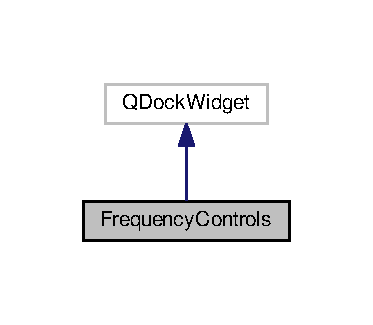
\includegraphics[width=179pt]{class_frequency_controls__inherit__graph}
\end{center}
\end{figure}


Collaboration diagram for Frequency\+Controls\+:\nopagebreak
\begin{figure}[H]
\begin{center}
\leavevmode
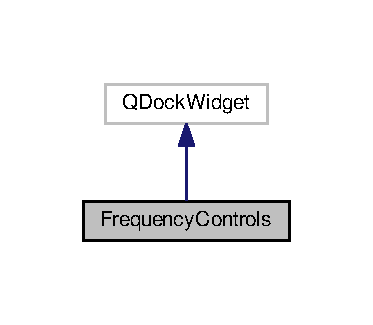
\includegraphics[width=179pt]{class_frequency_controls__coll__graph}
\end{center}
\end{figure}
\subsection*{Public Slots}
\begin{DoxyCompactItemize}
\item 
void {\bfseries Set\+Freq\+Span} (int span)\hypertarget{class_frequency_controls_a88109da989b014a69677728e96bb6a8a}{}\label{class_frequency_controls_a88109da989b014a69677728e96bb6a8a}

\item 
void {\bfseries Set\+Min\+Max} (std\+::pair$<$ int, int $>$ vals)\hypertarget{class_frequency_controls_acf2eee8710eac492be4004217fbbafd1}{}\label{class_frequency_controls_acf2eee8710eac492be4004217fbbafd1}

\end{DoxyCompactItemize}
\subsection*{Signals}
\begin{DoxyCompactItemize}
\item 
void {\bfseries Min\+Set} (double min\+\_\+val)\hypertarget{class_frequency_controls_a3544c74823a7aaabc9a0779ae839eb7f}{}\label{class_frequency_controls_a3544c74823a7aaabc9a0779ae839eb7f}

\item 
void {\bfseries Max\+Set} (double max\+\_\+val)\hypertarget{class_frequency_controls_ad8606de91f4ec71aa8011f658da35a4e}{}\label{class_frequency_controls_ad8606de91f4ec71aa8011f658da35a4e}

\item 
void {\bfseries Unit\+Selected} (Q\+String units)\hypertarget{class_frequency_controls_a5b873965eb03064dbcf713d0c66126d0}{}\label{class_frequency_controls_a5b873965eb03064dbcf713d0c66126d0}

\item 
void {\bfseries Span\+Set} (int span\+\_\+val)\hypertarget{class_frequency_controls_aef534d12777d179c45b59a47c8c1b431}{}\label{class_frequency_controls_aef534d12777d179c45b59a47c8c1b431}

\item 
void {\bfseries Center\+Set} (int cent\+\_\+val)\hypertarget{class_frequency_controls_afd8a0e6ada7b9063e15d55c9c6b562cb}{}\label{class_frequency_controls_afd8a0e6ada7b9063e15d55c9c6b562cb}

\end{DoxyCompactItemize}
\subsection*{Public Member Functions}
\begin{DoxyCompactItemize}
\item 
{\bfseries Frequency\+Controls} (Q\+Widget $\ast$parent=0)\hypertarget{class_frequency_controls_a41928b0575667ca2677e824a0907285b}{}\label{class_frequency_controls_a41928b0575667ca2677e824a0907285b}

\end{DoxyCompactItemize}


The documentation for this class was generated from the following files\+:\begin{DoxyCompactItemize}
\item 
/home/bephillips2/\+Qt-\/\+Projects/\+Electric\+\_\+\+Tiger\+\_\+\+D\+A\+Q/\+Panels/\+Graphic\+Objects/frequencycontrols.\+h\item 
/home/bephillips2/\+Qt-\/\+Projects/\+Electric\+\_\+\+Tiger\+\_\+\+D\+A\+Q/\+Panels/\+Graphic\+Objects/frequencycontrols.\+cpp\end{DoxyCompactItemize}

\hypertarget{class_instrument_view}{}\section{Instrument\+View Class Reference}
\label{class_instrument_view}\index{Instrument\+View@{Instrument\+View}}


Inheritance diagram for Instrument\+View\+:\nopagebreak
\begin{figure}[H]
\begin{center}
\leavevmode
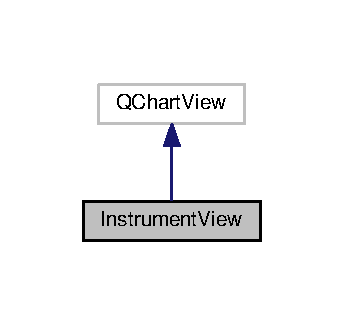
\includegraphics[width=165pt]{class_instrument_view__inherit__graph}
\end{center}
\end{figure}


Collaboration diagram for Instrument\+View\+:\nopagebreak
\begin{figure}[H]
\begin{center}
\leavevmode
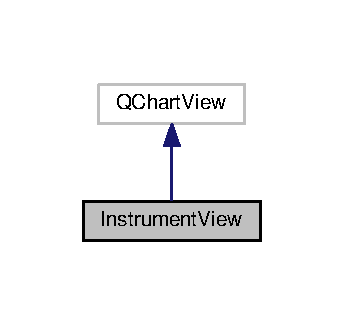
\includegraphics[width=165pt]{class_instrument_view__coll__graph}
\end{center}
\end{figure}
\subsection*{Public Slots}
\begin{DoxyCompactItemize}
\item 
void {\bfseries Set\+Frequency\+Min} (double min\+\_\+frequency)\hypertarget{class_instrument_view_ab91cbc99522a6045249bffacefd41514}{}\label{class_instrument_view_ab91cbc99522a6045249bffacefd41514}

\item 
void {\bfseries Set\+Power\+Min} (double min\+\_\+power)\hypertarget{class_instrument_view_a799847cc22b7e60d9fad7786b43e1b38}{}\label{class_instrument_view_a799847cc22b7e60d9fad7786b43e1b38}

\item 
void {\bfseries Set\+Frequency\+Max} (double max\+\_\+frequency)\hypertarget{class_instrument_view_a4e0fa885d57a9588bda4373bcb2568c3}{}\label{class_instrument_view_a4e0fa885d57a9588bda4373bcb2568c3}

\item 
void {\bfseries Set\+Power\+Max} (double max\+\_\+power)\hypertarget{class_instrument_view_ab8479bd6bc1690b687e6edafb8470cb3}{}\label{class_instrument_view_ab8479bd6bc1690b687e6edafb8470cb3}

\item 
void {\bfseries Update\+Signal} (std\+::vector$<$ double $>$ data, double freq\+\_\+span)\hypertarget{class_instrument_view_aeedb3cab5a13eef6127b73976f50c584}{}\label{class_instrument_view_aeedb3cab5a13eef6127b73976f50c584}

\end{DoxyCompactItemize}
\subsection*{Signals}
\begin{DoxyCompactItemize}
\item 
void {\bfseries Signal\+Changed} ()\hypertarget{class_instrument_view_a34307a11aea62e2bde7b56b44d118193}{}\label{class_instrument_view_a34307a11aea62e2bde7b56b44d118193}

\end{DoxyCompactItemize}
\subsection*{Public Member Functions}
\begin{DoxyCompactItemize}
\item 
{\bfseries Instrument\+View} (Q\+String title, Q\+Widget $\ast$parent=0)\hypertarget{class_instrument_view_ad5895e0a5192e456d2fc4d33c72c5c8c}{}\label{class_instrument_view_ad5895e0a5192e456d2fc4d33c72c5c8c}

\item 
{\footnotesize template$<$class T , typename F $>$ }\\void {\bfseries Plot\+Auto\+Scale} (const T \&y\+\_\+signal\+\_\+elements, F x\+\_\+frequency\+\_\+range)\hypertarget{class_instrument_view_a8bb3f9c2ccf3dfd8e462efc0bd7535ab}{}\label{class_instrument_view_a8bb3f9c2ccf3dfd8e462efc0bd7535ab}

\item 
{\footnotesize template$<$class T $>$ }\\void {\bfseries Plot} (const T \&y\+\_\+signal\+\_\+elements, double x\+\_\+frequency\+\_\+range)\hypertarget{class_instrument_view_a9cbc2653dc03c2913ef967052d6e16bd}{}\label{class_instrument_view_a9cbc2653dc03c2913ef967052d6e16bd}

\end{DoxyCompactItemize}


The documentation for this class was generated from the following files\+:\begin{DoxyCompactItemize}
\item 
/home/bephillips2/\+Qt-\/\+Projects/\+Electric\+\_\+\+Tiger\+\_\+\+D\+A\+Q/\+Panels/\+Instrument\+View/instrumentview.\+h\item 
/home/bephillips2/\+Qt-\/\+Projects/\+Electric\+\_\+\+Tiger\+\_\+\+D\+A\+Q/\+Panels/\+Instrument\+View/instrumentview.\+cpp\end{DoxyCompactItemize}

\hypertarget{class_main_window}{}\section{Main\+Window Class Reference}
\label{class_main_window}\index{Main\+Window@{Main\+Window}}


Inheritance diagram for Main\+Window\+:\nopagebreak
\begin{figure}[H]
\begin{center}
\leavevmode
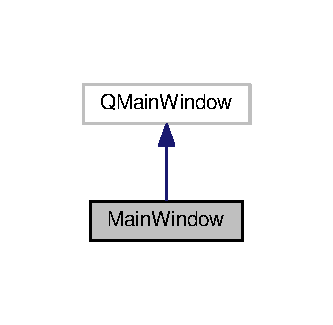
\includegraphics[width=160pt]{class_main_window__inherit__graph}
\end{center}
\end{figure}


Collaboration diagram for Main\+Window\+:\nopagebreak
\begin{figure}[H]
\begin{center}
\leavevmode
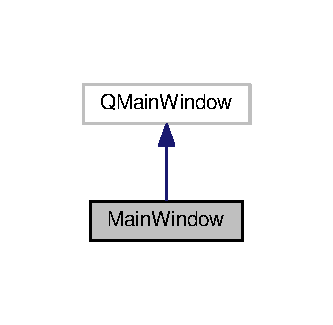
\includegraphics[width=160pt]{class_main_window__coll__graph}
\end{center}
\end{figure}
\subsection*{Public Member Functions}
\begin{DoxyCompactItemize}
\item 
{\bfseries Main\+Window} (Q\+Widget $\ast$parent=0)\hypertarget{class_main_window_a8b244be8b7b7db1b08de2a2acb9409db}{}\label{class_main_window_a8b244be8b7b7db1b08de2a2acb9409db}

\item 
void {\bfseries Set\+Spectrum\+Analyzer\+View} (\hyperlink{class_spectrum_analyzer}{Spectrum\+Analyzer} $\ast$spec\+\_\+analyzer)\hypertarget{class_main_window_a682438fcbf5c684e47a6a089477d8a8a}{}\label{class_main_window_a682438fcbf5c684e47a6a089477d8a8a}

\item 
void {\bfseries Set\+Network\+Analyzer\+View} (\hyperlink{class_instrument_view}{Instrument\+View} $\ast$network\+\_\+analyzer)\hypertarget{class_main_window_aff3b43153f014e8aac712dbeae7eb255}{}\label{class_main_window_aff3b43153f014e8aac712dbeae7eb255}

\item 
void {\bfseries Set\+Combo\+Status} (\hyperlink{class_combo_status_panel}{Combo\+Status\+Panel} $\ast$status\+\_\+panel)\hypertarget{class_main_window_a656a32c45bc35ea5a66573ecdf49498a}{}\label{class_main_window_a656a32c45bc35ea5a66573ecdf49498a}

\end{DoxyCompactItemize}


The documentation for this class was generated from the following files\+:\begin{DoxyCompactItemize}
\item 
/home/bephillips2/\+Qt-\/\+Projects/\+Electric\+\_\+\+Tiger\+\_\+\+D\+A\+Q/\+Windows/mainwindow.\+h\item 
/home/bephillips2/\+Qt-\/\+Projects/\+Electric\+\_\+\+Tiger\+\_\+\+D\+A\+Q/\+Windows/mainwindow.\+cpp\end{DoxyCompactItemize}

\hypertarget{classmode__track__failure}{}\section{mode\+\_\+track\+\_\+failure Class Reference}
\label{classmode__track__failure}\index{mode\+\_\+track\+\_\+failure@{mode\+\_\+track\+\_\+failure}}


Inheritance diagram for mode\+\_\+track\+\_\+failure\+:\nopagebreak
\begin{figure}[H]
\begin{center}
\leavevmode
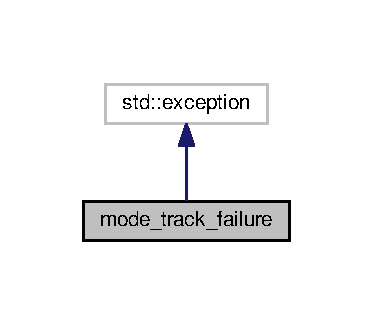
\includegraphics[width=179pt]{classmode__track__failure__inherit__graph}
\end{center}
\end{figure}


Collaboration diagram for mode\+\_\+track\+\_\+failure\+:\nopagebreak
\begin{figure}[H]
\begin{center}
\leavevmode
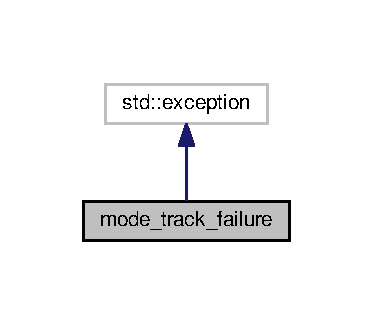
\includegraphics[width=179pt]{classmode__track__failure__coll__graph}
\end{center}
\end{figure}
\subsection*{Public Member Functions}
\begin{DoxyCompactItemize}
\item 
{\bfseries mode\+\_\+track\+\_\+failure} (const char $\ast$message)\hypertarget{classmode__track__failure_a3636c3b5e513a98e420d7b769803fb07}{}\label{classmode__track__failure_a3636c3b5e513a98e420d7b769803fb07}

\item 
const char $\ast$ {\bfseries what} () const   throw ()\hypertarget{classmode__track__failure_a9a6a0afd0b4b1f675d5e3ab17313d937}{}\label{classmode__track__failure_a9a6a0afd0b4b1f675d5e3ab17313d937}

\end{DoxyCompactItemize}


The documentation for this class was generated from the following file\+:\begin{DoxyCompactItemize}
\item 
/home/bephillips2/\+Qt-\/\+Projects/\+Electric\+\_\+\+Tiger\+\_\+\+D\+A\+Q/\+Mode\+Tracker/mode\+\_\+track\+\_\+failure.\+h\end{DoxyCompactItemize}

\hypertarget{class_mode_track}{}\section{Mode\+Track Class Reference}
\label{class_mode_track}\index{Mode\+Track@{Mode\+Track}}


Base Class for mode tracking algorithims; designed to be wrapped with Swig and called from Python module.  




{\ttfamily \#include $<$modetrack.\+h$>$}

\subsection*{Public Member Functions}
\begin{DoxyCompactItemize}
\item 
void \hyperlink{class_mode_track_a3163e67113b3a93cb9fde40cba8dc813}{Set\+Background} (const std\+::vector$<$ \hyperlink{structdata__triple}{data\+\_\+triple}$<$ double $>$ $>$ \&background\+\_\+list)
\begin{DoxyCompactList}\small\item\em Set background data which will be subtracted from each measurement. \end{DoxyCompactList}\item 
double \hyperlink{class_mode_track_a2b3cc468fae5bca487871ad2b71fc974}{Get\+Peaks\+Gauss} (const std\+::vector$<$ \hyperlink{structdata__triple}{data\+\_\+triple}$<$ double $>$ $>$ \&power\+\_\+list, int mod\+\_\+number)
\begin{DoxyCompactList}\small\item\em Identify minima peaks in a list of power data using Gaussian filtering. \end{DoxyCompactList}\item 
double \hyperlink{class_mode_track_a974e74566b3baf1343d5942a6af7445e}{Get\+Peaks\+Bi\+Lat} (const std\+::vector$<$ \hyperlink{structdata__triple}{data\+\_\+triple}$<$ double $>$ $>$ \&power\+\_\+list, int mod\+\_\+number)
\begin{DoxyCompactList}\small\item\em Identify minima peaks in a list of power data using Bilateral filtering. \end{DoxyCompactList}\item 
double \hyperlink{class_mode_track_ab471ed8393b84636edb129d1c77b4df4}{Get\+Max\+Peak} (const std\+::vector$<$ \hyperlink{structdata__triple}{data\+\_\+triple}$<$ double $>$ $>$ \&power\+\_\+list)
\begin{DoxyCompactList}\small\item\em Find a local maximum in a list of data. \end{DoxyCompactList}\item 
void {\bfseries Set\+Lower\+Bound} (double frequency)\hypertarget{class_mode_track_a99eeeb6757873474994a61dbd7e31e43}{}\label{class_mode_track_a99eeeb6757873474994a61dbd7e31e43}

\item 
void {\bfseries Set\+Upper\+Bound} (double frequency)\hypertarget{class_mode_track_a7b7a1977d0cdacf2533581c82707e018}{}\label{class_mode_track_a7b7a1977d0cdacf2533581c82707e018}

\end{DoxyCompactItemize}


\subsection{Detailed Description}
Base Class for mode tracking algorithims; designed to be wrapped with Swig and called from Python module. 

\subsection{Member Function Documentation}
\index{Mode\+Track@{Mode\+Track}!Get\+Max\+Peak@{Get\+Max\+Peak}}
\index{Get\+Max\+Peak@{Get\+Max\+Peak}!Mode\+Track@{Mode\+Track}}
\subsubsection[{\texorpdfstring{Get\+Max\+Peak(const std\+::vector$<$ data\+\_\+triple$<$ double $>$ $>$ \&power\+\_\+list)}{GetMaxPeak(const std::vector< data_triple< double > > &power_list)}}]{\setlength{\rightskip}{0pt plus 5cm}double Mode\+Track\+::\+Get\+Max\+Peak (
\begin{DoxyParamCaption}
\item[{const std\+::vector$<$ {\bf data\+\_\+triple}$<$ double $>$ $>$ \&}]{power\+\_\+list}
\end{DoxyParamCaption}
)}\hypertarget{class_mode_track_ab471ed8393b84636edb129d1c77b4df4}{}\label{class_mode_track_ab471ed8393b84636edb129d1c77b4df4}


Find a local maximum in a list of data. 

This method applies the same Gaussian Blur/\+Derivative filter combination that \textquotesingle{}Get\+Peaks\textquotesingle{} uses, but does not make reference to the estimated peak positions. If multiple peaks are identified take the one with the highest overall value. This function is designed to be called when identifying peaks when looking at a transmission measurement.

\begin{DoxyReturn}{Returns}
Frequency of maxima, if one is found. Otherwise return value will be 0. 
\end{DoxyReturn}
\index{Mode\+Track@{Mode\+Track}!Get\+Peaks\+Bi\+Lat@{Get\+Peaks\+Bi\+Lat}}
\index{Get\+Peaks\+Bi\+Lat@{Get\+Peaks\+Bi\+Lat}!Mode\+Track@{Mode\+Track}}
\subsubsection[{\texorpdfstring{Get\+Peaks\+Bi\+Lat(const std\+::vector$<$ data\+\_\+triple$<$ double $>$ $>$ \&power\+\_\+list, int mod\+\_\+number)}{GetPeaksBiLat(const std::vector< data_triple< double > > &power_list, int mod_number)}}]{\setlength{\rightskip}{0pt plus 5cm}double Mode\+Track\+::\+Get\+Peaks\+Bi\+Lat (
\begin{DoxyParamCaption}
\item[{const std\+::vector$<$ {\bf data\+\_\+triple}$<$ double $>$ $>$ \&}]{power\+\_\+list, }
\item[{int}]{mod\+\_\+number}
\end{DoxyParamCaption}
)}\hypertarget{class_mode_track_a974e74566b3baf1343d5942a6af7445e}{}\label{class_mode_track_a974e74566b3baf1343d5942a6af7445e}


Identify minima peaks in a list of power data using Bilateral filtering. 

This function is very similar to \hyperlink{class_mode_track_a2b3cc468fae5bca487871ad2b71fc974}{Get\+Peaks\+Gauss()} except for the method that is used to filter data. This function makes use of a Bilateral filter for data pre-\/processing.

See \href{https://users.cs.duke.edu/~tomasi/papers/tomasi/tomasiIccv98.pdf}{\tt https\+://users.\+cs.\+duke.\+edu/$\sim$tomasi/papers/tomasi/tomasi\+Iccv98.\+pdf} for more details.


\begin{DoxyParams}{Parameters}
{\em data\+\_\+str} & string containing power data that should be searched through. Needs to be in the a list of values seperated by commas, eg $ \{p_1,p_2,...,p_n\}$\\
\hline
{\em mode\+\_\+number} & Identify which mode should be tracked. Choices are 0,1,2 and 3.\\
\hline
\end{DoxyParams}
\begin{DoxyReturn}{Returns}
The frequency of the requested mode in M\+Hz. If the requested mode was not found a value of 0 will be returned. 
\end{DoxyReturn}
\index{Mode\+Track@{Mode\+Track}!Get\+Peaks\+Gauss@{Get\+Peaks\+Gauss}}
\index{Get\+Peaks\+Gauss@{Get\+Peaks\+Gauss}!Mode\+Track@{Mode\+Track}}
\subsubsection[{\texorpdfstring{Get\+Peaks\+Gauss(const std\+::vector$<$ data\+\_\+triple$<$ double $>$ $>$ \&power\+\_\+list, int mod\+\_\+number)}{GetPeaksGauss(const std::vector< data_triple< double > > &power_list, int mod_number)}}]{\setlength{\rightskip}{0pt plus 5cm}double Mode\+Track\+::\+Get\+Peaks\+Gauss (
\begin{DoxyParamCaption}
\item[{const std\+::vector$<$ {\bf data\+\_\+triple}$<$ double $>$ $>$ \&}]{power\+\_\+list, }
\item[{int}]{mod\+\_\+number}
\end{DoxyParamCaption}
)}\hypertarget{class_mode_track_a2b3cc468fae5bca487871ad2b71fc974}{}\label{class_mode_track_a2b3cc468fae5bca487871ad2b71fc974}


Identify minima peaks in a list of power data using Gaussian filtering. 

This function is designed to be called by the main control code during data taking. The main control program will collect reflection measurements and call this function to identify the position of the mode of desire.


\begin{DoxyParams}{Parameters}
{\em data\+\_\+str} & string containing power data that should be searched through. Needs to be in the a list of values seperated by commas, eg $ \{p_1,p_2,...,p_n\}$\\
\hline
{\em mode\+\_\+number} & Identify which mode should be tracked. Choices are 0,1,2 and 3.\\
\hline
\end{DoxyParams}
\begin{DoxyReturn}{Returns}
The frequency of the requested mode in M\+Hz. If the requested mode was not found a value of 0 will be returned. 
\end{DoxyReturn}
\index{Mode\+Track@{Mode\+Track}!Set\+Background@{Set\+Background}}
\index{Set\+Background@{Set\+Background}!Mode\+Track@{Mode\+Track}}
\subsubsection[{\texorpdfstring{Set\+Background(const std\+::vector$<$ data\+\_\+triple$<$ double $>$ $>$ \&background\+\_\+list)}{SetBackground(const std::vector< data_triple< double > > &background_list)}}]{\setlength{\rightskip}{0pt plus 5cm}void Mode\+Track\+::\+Set\+Background (
\begin{DoxyParamCaption}
\item[{const std\+::vector$<$ {\bf data\+\_\+triple}$<$ double $>$ $>$ \&}]{background\+\_\+list}
\end{DoxyParamCaption}
)}\hypertarget{class_mode_track_a3163e67113b3a93cb9fde40cba8dc813}{}\label{class_mode_track_a3163e67113b3a93cb9fde40cba8dc813}


Set background data which will be subtracted from each measurement. 


\begin{DoxyParams}{Parameters}
{\em background\+\_\+str} & string of power values seperated by commas, eg $ \{p_1,p_2,...,p_n\}$ \\
\hline
\end{DoxyParams}


The documentation for this class was generated from the following files\+:\begin{DoxyCompactItemize}
\item 
/home/bephillips2/\+Qt-\/\+Projects/\+Electric\+\_\+\+Tiger\+\_\+\+D\+A\+Q/\+Mode\+Tracker/modetrack.\+h\item 
/home/bephillips2/\+Qt-\/\+Projects/\+Electric\+\_\+\+Tiger\+\_\+\+D\+A\+Q/\+Mode\+Tracker/modetrack.\+cpp\end{DoxyCompactItemize}

\hypertarget{class_mode_traits}{}\section{Mode\+Traits Class Reference}
\label{class_mode_traits}\index{Mode\+Traits@{Mode\+Traits}}
\subsection*{Public Member Functions}
\begin{DoxyCompactItemize}
\item 
{\bfseries Mode\+Traits} (const std\+::vector$<$ \hyperlink{structdata__triple}{data\+\_\+triple}$<$ double $>$ $>$ \&data\+\_\+values)\hypertarget{class_mode_traits_ade9c65b78b5140f3fd2eaabcd38d1837}{}\label{class_mode_traits_ade9c65b78b5140f3fd2eaabcd38d1837}

\item 
double {\bfseries Q} ()\hypertarget{class_mode_traits_a83b44ff9b0e9db253c7cd13b1e51a736}{}\label{class_mode_traits_a83b44ff9b0e9db253c7cd13b1e51a736}

\item 
double {\bfseries f0} ()\hypertarget{class_mode_traits_a903f06c1d611514e42869f6d6b1e387f}{}\label{class_mode_traits_a903f06c1d611514e42869f6d6b1e387f}

\end{DoxyCompactItemize}


The documentation for this class was generated from the following files\+:\begin{DoxyCompactItemize}
\item 
/home/bephillips2/\+Qt-\/\+Projects/\+Electric\+\_\+\+Tiger\+\_\+\+D\+A\+Q/\+Mode\+Characterization/modecharacterization.\+h\item 
/home/bephillips2/\+Qt-\/\+Projects/\+Electric\+\_\+\+Tiger\+\_\+\+D\+A\+Q/\+Mode\+Characterization/modecharacterization.\+cpp\end{DoxyCompactItemize}

\hypertarget{class_network_analyzer}{}\section{Network\+Analyzer Class Reference}
\label{class_network_analyzer}\index{Network\+Analyzer@{Network\+Analyzer}}


Object to communicate with the H\+P8757 C Network Analyzer.  




{\ttfamily \#include $<$network\+\_\+analyzer.\+h$>$}



Inheritance diagram for Network\+Analyzer\+:\nopagebreak
\begin{figure}[H]
\begin{center}
\leavevmode
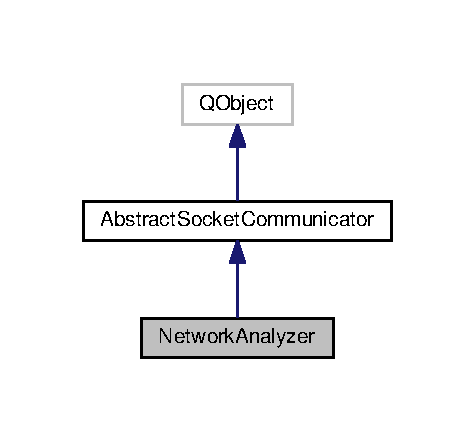
\includegraphics[width=228pt]{class_network_analyzer__inherit__graph}
\end{center}
\end{figure}


Collaboration diagram for Network\+Analyzer\+:\nopagebreak
\begin{figure}[H]
\begin{center}
\leavevmode
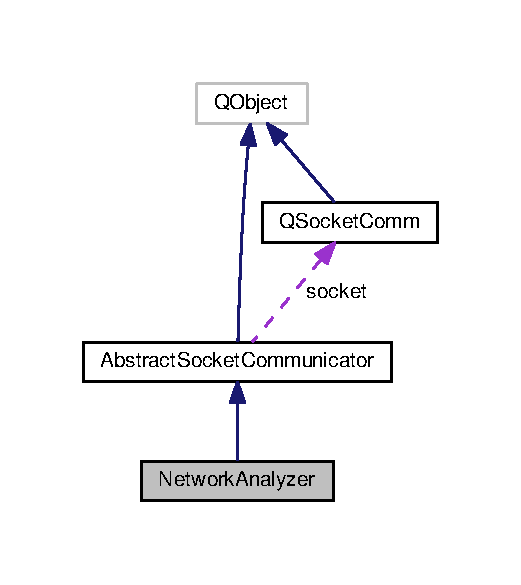
\includegraphics[width=250pt]{class_network_analyzer__coll__graph}
\end{center}
\end{figure}
\subsection*{Public Member Functions}
\begin{DoxyCompactItemize}
\item 
{\bfseries Network\+Analyzer} (std\+::string ip\+\_\+addr, uint port\+\_\+number, uint points, double span, double power, Q\+Object $\ast$parent=0)\hypertarget{class_network_analyzer_a99a9eb7f1bfd2819e695a342e2b9be98}{}\label{class_network_analyzer_a99a9eb7f1bfd2819e695a342e2b9be98}

\item 
\hyperlink{class_network_analyzer}{Network\+Analyzer} \& {\bfseries operator=} (const \hyperlink{class_network_analyzer}{Network\+Analyzer} \&)=delete\hypertarget{class_network_analyzer_a2785c012d28fb621e7218a9e471716e3}{}\label{class_network_analyzer_a2785c012d28fb621e7218a9e471716e3}

\item 
std\+::vector$<$ double $>$ {\bfseries Take\+Data\+Multiple} ()\hypertarget{class_network_analyzer_a667cf86a80639bb57c67061b7c9df210}{}\label{class_network_analyzer_a667cf86a80639bb57c67061b7c9df210}

\item 
std\+::vector$<$ double $>$ \hyperlink{class_network_analyzer_aa7ae9c649f4d7a5828e2d24ad8dee65d}{Take\+Data\+Single} ()
\begin{DoxyCompactList}\small\item\em Collect a single power spectrum from the Network Analyzer. \end{DoxyCompactList}\item 
void {\bfseries Set\+Frequency\+Window} (double frequency, double frequency\+\_\+span)\hypertarget{class_network_analyzer_a65864fe6142eadfd8e3e976e592e4bf0}{}\label{class_network_analyzer_a65864fe6142eadfd8e3e976e592e4bf0}

\item 
void {\bfseries Set\+Frequency\+Span} (double frequency\+\_\+span)\hypertarget{class_network_analyzer_a5d986f4eb0ed10030ba02ef43b65ac30}{}\label{class_network_analyzer_a5d986f4eb0ed10030ba02ef43b65ac30}

\item 
void \hyperlink{class_network_analyzer_a6d4e76a043fd30788167c4c0e187ed00}{Turn\+On\+R\+F\+Source} ()\hypertarget{class_network_analyzer_a6d4e76a043fd30788167c4c0e187ed00}{}\label{class_network_analyzer_a6d4e76a043fd30788167c4c0e187ed00}

\begin{DoxyCompactList}\small\item\em Turn the RF source on, at whatever power it was set to most recently. \end{DoxyCompactList}\item 
void \hyperlink{class_network_analyzer_aeeb9823df08d7b602d524583fcc94c26}{Turn\+Off\+R\+F\+Source} ()\hypertarget{class_network_analyzer_aeeb9823df08d7b602d524583fcc94c26}{}\label{class_network_analyzer_aeeb9823df08d7b602d524583fcc94c26}

\begin{DoxyCompactList}\small\item\em Turn the RF source off. \end{DoxyCompactList}\end{DoxyCompactItemize}
\subsection*{Additional Inherited Members}


\subsection{Detailed Description}
Object to communicate with the H\+P8757 C Network Analyzer. 

\subsection{Member Function Documentation}
\index{Network\+Analyzer@{Network\+Analyzer}!Take\+Data\+Single@{Take\+Data\+Single}}
\index{Take\+Data\+Single@{Take\+Data\+Single}!Network\+Analyzer@{Network\+Analyzer}}
\subsubsection[{\texorpdfstring{Take\+Data\+Single()}{TakeDataSingle()}}]{\setlength{\rightskip}{0pt plus 5cm}std\+::vector$<$ double $>$ Network\+Analyzer\+::\+Take\+Data\+Single (
\begin{DoxyParamCaption}
{}
\end{DoxyParamCaption}
)}\hypertarget{class_network_analyzer_aa7ae9c649f4d7a5828e2d24ad8dee65d}{}\label{class_network_analyzer_aa7ae9c649f4d7a5828e2d24ad8dee65d}


Collect a single power spectrum from the Network Analyzer. 

Settings will be whatever the Network Analyzer was set to when this function is called. \begin{DoxyReturn}{Returns}

\end{DoxyReturn}


The documentation for this class was generated from the following files\+:\begin{DoxyCompactItemize}
\item 
/home/bephillips2/\+Qt-\/\+Projects/\+Electric\+\_\+\+Tiger\+\_\+\+D\+A\+Q/\+Socket\+Communicators/\+Network\+Analyzer/network\+\_\+analyzer.\+h\item 
/home/bephillips2/\+Qt-\/\+Projects/\+Electric\+\_\+\+Tiger\+\_\+\+D\+A\+Q/\+Socket\+Communicators/\+Network\+Analyzer/network\+\_\+analyzer.\+cpp\end{DoxyCompactItemize}

\hypertarget{struct_plain_data_param}{}\section{Plain\+Data\+Param$<$ T $>$ Struct Template Reference}
\label{struct_plain_data_param}\index{Plain\+Data\+Param$<$ T $>$@{Plain\+Data\+Param$<$ T $>$}}
\subsection*{Public Member Functions}
\begin{DoxyCompactItemize}
\item 
{\bfseries Plain\+Data\+Param} (std\+::string name, T val)\hypertarget{struct_plain_data_param_a794c26a7b671bb3c3ef52e7c7ba447a5}{}\label{struct_plain_data_param_a794c26a7b671bb3c3ef52e7c7ba447a5}

\end{DoxyCompactItemize}
\subsection*{Public Attributes}
\begin{DoxyCompactItemize}
\item 
const std\+::string {\bfseries data\+\_\+name}\hypertarget{struct_plain_data_param_a2376eb9c88951f9648048b4d8c46968b}{}\label{struct_plain_data_param_a2376eb9c88951f9648048b4d8c46968b}

\item 
const T {\bfseries data\+\_\+value}\hypertarget{struct_plain_data_param_a725d21ff8568129d46a516944b83ca6a}{}\label{struct_plain_data_param_a725d21ff8568129d46a516944b83ca6a}

\end{DoxyCompactItemize}
\subsection*{Friends}
\begin{DoxyCompactItemize}
\item 
std\+::ostream \& {\bfseries operator$<$$<$} (std\+::ostream \&stream, \hyperlink{struct_plain_data_param}{Plain\+Data\+Param} \&param)\hypertarget{struct_plain_data_param_a72df40b826bf228821a4f0e488fde836}{}\label{struct_plain_data_param_a72df40b826bf228821a4f0e488fde836}

\end{DoxyCompactItemize}


The documentation for this struct was generated from the following file\+:\begin{DoxyCompactItemize}
\item 
/home/bephillips2/\+Qt-\/\+Projects/\+Electric\+\_\+\+Tiger\+\_\+\+D\+A\+Q/\+Config\+Processor/configprocessor.\+h\end{DoxyCompactItemize}

\hypertarget{class_power_controls}{}\section{Power\+Controls Class Reference}
\label{class_power_controls}\index{Power\+Controls@{Power\+Controls}}


Inheritance diagram for Power\+Controls\+:\nopagebreak
\begin{figure}[H]
\begin{center}
\leavevmode
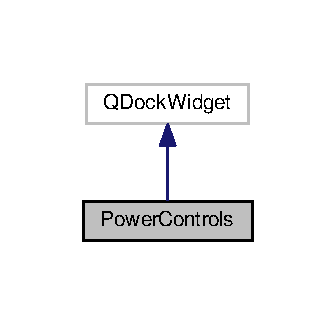
\includegraphics[width=161pt]{class_power_controls__inherit__graph}
\end{center}
\end{figure}


Collaboration diagram for Power\+Controls\+:\nopagebreak
\begin{figure}[H]
\begin{center}
\leavevmode
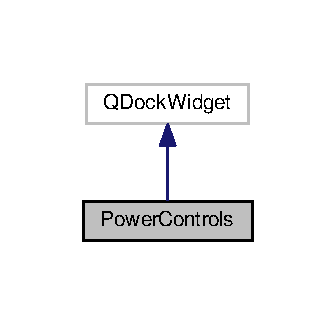
\includegraphics[width=161pt]{class_power_controls__coll__graph}
\end{center}
\end{figure}
\subsection*{Public Slots}
\begin{DoxyCompactItemize}
\item 
void {\bfseries Set\+Freq\+Span} (int span)\hypertarget{class_power_controls_a9bd193055b86e97e51d96912271fffe5}{}\label{class_power_controls_a9bd193055b86e97e51d96912271fffe5}

\item 
void {\bfseries Set\+Min\+Max} (std\+::pair$<$ int, int $>$ vals)\hypertarget{class_power_controls_afa8e34d9a376e9abc0839e3caafa6ab9}{}\label{class_power_controls_afa8e34d9a376e9abc0839e3caafa6ab9}

\end{DoxyCompactItemize}
\subsection*{Signals}
\begin{DoxyCompactItemize}
\item 
void {\bfseries Min\+Set} (double min\+\_\+val)\hypertarget{class_power_controls_ab9a1d9f89f194471d0e31f6dad01086a}{}\label{class_power_controls_ab9a1d9f89f194471d0e31f6dad01086a}

\item 
void {\bfseries Max\+Set} (double max\+\_\+val)\hypertarget{class_power_controls_aef88de9bf3ae6738020c9334ee79e857}{}\label{class_power_controls_aef88de9bf3ae6738020c9334ee79e857}

\item 
void {\bfseries Unit\+Selected} (Q\+String units)\hypertarget{class_power_controls_a6077789456f1780b9f86569256334a38}{}\label{class_power_controls_a6077789456f1780b9f86569256334a38}

\item 
void {\bfseries Span\+Set} (int span\+\_\+val)\hypertarget{class_power_controls_ad146203ff843dd336cca6838be0aa9b4}{}\label{class_power_controls_ad146203ff843dd336cca6838be0aa9b4}

\item 
void {\bfseries Center\+Set} (int cent\+\_\+val)\hypertarget{class_power_controls_a79b389c9c31f94eb5b0ae8fc771b1c7d}{}\label{class_power_controls_a79b389c9c31f94eb5b0ae8fc771b1c7d}

\item 
void {\bfseries Selected\+Volts} ()\hypertarget{class_power_controls_a3da815aa3bab7ba24273c1eac5ee32e5}{}\label{class_power_controls_a3da815aa3bab7ba24273c1eac5ee32e5}

\item 
void {\bfseries Selectedd\+Bm} ()\hypertarget{class_power_controls_a8a2eb48c9ed37db4cf934f022b7c556f}{}\label{class_power_controls_a8a2eb48c9ed37db4cf934f022b7c556f}

\item 
void {\bfseries Auto\+Scale\+On} ()\hypertarget{class_power_controls_a6c0db9226b82cbf54f50f6e6cc630fb2}{}\label{class_power_controls_a6c0db9226b82cbf54f50f6e6cc630fb2}

\item 
void {\bfseries Auto\+Scale\+Off} ()\hypertarget{class_power_controls_a374af54d153a4b0381b3ce1e73e7864f}{}\label{class_power_controls_a374af54d153a4b0381b3ce1e73e7864f}

\end{DoxyCompactItemize}
\subsection*{Public Member Functions}
\begin{DoxyCompactItemize}
\item 
{\bfseries Power\+Controls} (Q\+Widget $\ast$parent=0)\hypertarget{class_power_controls_a73bb29ad05d93d0d945596b02b3a058a}{}\label{class_power_controls_a73bb29ad05d93d0d945596b02b3a058a}

\end{DoxyCompactItemize}


The documentation for this class was generated from the following files\+:\begin{DoxyCompactItemize}
\item 
/home/bephillips2/\+Qt-\/\+Projects/\+Electric\+\_\+\+Tiger\+\_\+\+D\+A\+Q/\+Panels/\+Graphic\+Objects/chartscalecontrols.\+h\item 
/home/bephillips2/\+Qt-\/\+Projects/\+Electric\+\_\+\+Tiger\+\_\+\+D\+A\+Q/\+Panels/\+Graphic\+Objects/chartscalecontrols.\+cpp\end{DoxyCompactItemize}

\hypertarget{classetig_1_1_program}{}\section{etig\+:\+:Program Class Reference}
\label{classetig_1_1_program}\index{etig\+::\+Program@{etig\+::\+Program}}


Inheritance diagram for etig\+:\+:Program\+:\nopagebreak
\begin{figure}[H]
\begin{center}
\leavevmode
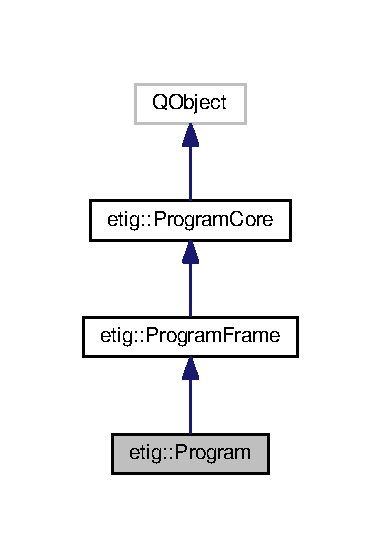
\includegraphics[width=183pt]{classetig_1_1_program__inherit__graph}
\end{center}
\end{figure}


Collaboration diagram for etig\+:\+:Program\+:\nopagebreak
\begin{figure}[H]
\begin{center}
\leavevmode
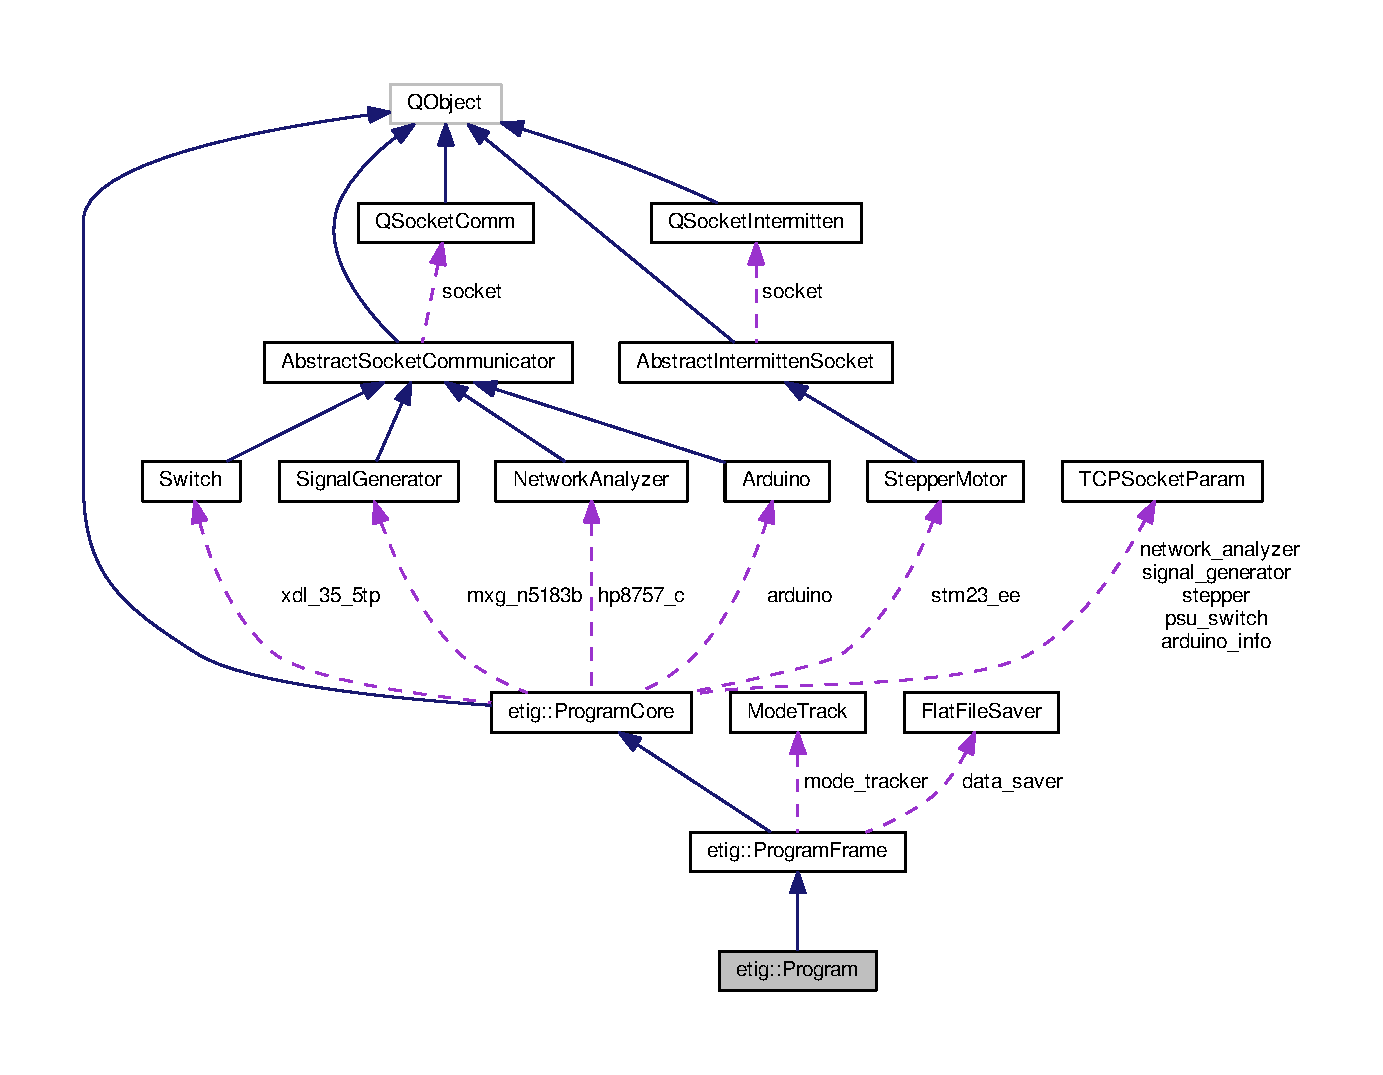
\includegraphics[width=350pt]{classetig_1_1_program__coll__graph}
\end{center}
\end{figure}
\subsection*{Public Slots}
\begin{DoxyCompactItemize}
\item 
void {\bfseries Run} ()\hypertarget{classetig_1_1_program_a15392fd26830cb264cff92092a48c874}{}\label{classetig_1_1_program_a15392fd26830cb264cff92092a48c874}

\item 
void {\bfseries Stop} ()\hypertarget{classetig_1_1_program_a5d144652844118b17dd8e591415365ac}{}\label{classetig_1_1_program_a5d144652844118b17dd8e591415365ac}

\end{DoxyCompactItemize}
\subsection*{Public Member Functions}
\begin{DoxyCompactItemize}
\item 
{\bfseries Program} (Q\+Object $\ast$parent=0)\hypertarget{classetig_1_1_program_a8c31dffc20c4394929dd300ac92972d7}{}\label{classetig_1_1_program_a8c31dffc20c4394929dd300ac92972d7}

\item 
double {\bfseries Find\+Mode\+Reflection} ()\hypertarget{classetig_1_1_program_a1299fec5e80b7d7eb1ca0cda7eb3119b}{}\label{classetig_1_1_program_a1299fec5e80b7d7eb1ca0cda7eb3119b}

\item 
double {\bfseries Find\+Mode\+Transmission} (double mode\+\_\+frequency)\hypertarget{classetig_1_1_program_ae5bc8e04ddd5ed957e1ace2f2bc3d5d9}{}\label{classetig_1_1_program_ae5bc8e04ddd5ed957e1ace2f2bc3d5d9}

\item 
data\+\_\+list {\bfseries Take\+Data} (double mode\+\_\+frequency)\hypertarget{classetig_1_1_program_ac01f0ba930b0bb450905c1377decfffa}{}\label{classetig_1_1_program_ac01f0ba930b0bb450905c1377decfffa}

\item 
void {\bfseries Save\+Power\+Spectrum} (const data\+\_\+list \&scan)\hypertarget{classetig_1_1_program_ab0cf10316e239d8c64299b70b4c383dd}{}\label{classetig_1_1_program_ab0cf10316e239d8c64299b70b4c383dd}

\item 
void {\bfseries Panic\+Clean\+Up} ()\hypertarget{classetig_1_1_program_af6162f08814e2c7e751fd0c3e9d986cb}{}\label{classetig_1_1_program_af6162f08814e2c7e751fd0c3e9d986cb}

\end{DoxyCompactItemize}
\subsection*{Additional Inherited Members}


The documentation for this class was generated from the following files\+:\begin{DoxyCompactItemize}
\item 
/home/bephillips2/\+Qt-\/\+Projects/\+Electric\+\_\+\+Tiger\+\_\+\+D\+A\+Q/\+Program/\+Program/program.\+h\item 
/home/bephillips2/\+Qt-\/\+Projects/\+Electric\+\_\+\+Tiger\+\_\+\+D\+A\+Q/\+Program/\+Program/program.\+cpp\end{DoxyCompactItemize}

\hypertarget{classetig_1_1_program_core}{}\section{etig\+:\+:Program\+Core Class Reference}
\label{classetig_1_1_program_core}\index{etig\+::\+Program\+Core@{etig\+::\+Program\+Core}}


Inheritance diagram for etig\+:\+:Program\+Core\+:\nopagebreak
\begin{figure}[H]
\begin{center}
\leavevmode
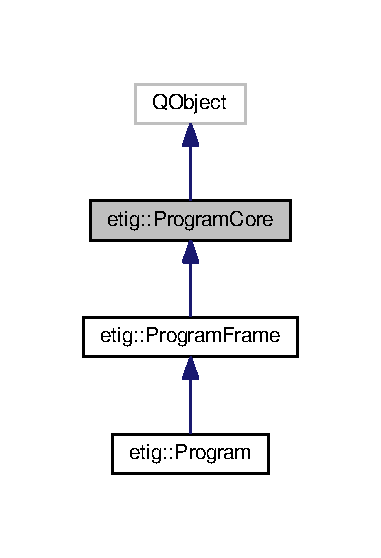
\includegraphics[width=183pt]{classetig_1_1_program_core__inherit__graph}
\end{center}
\end{figure}


Collaboration diagram for etig\+:\+:Program\+Core\+:\nopagebreak
\begin{figure}[H]
\begin{center}
\leavevmode
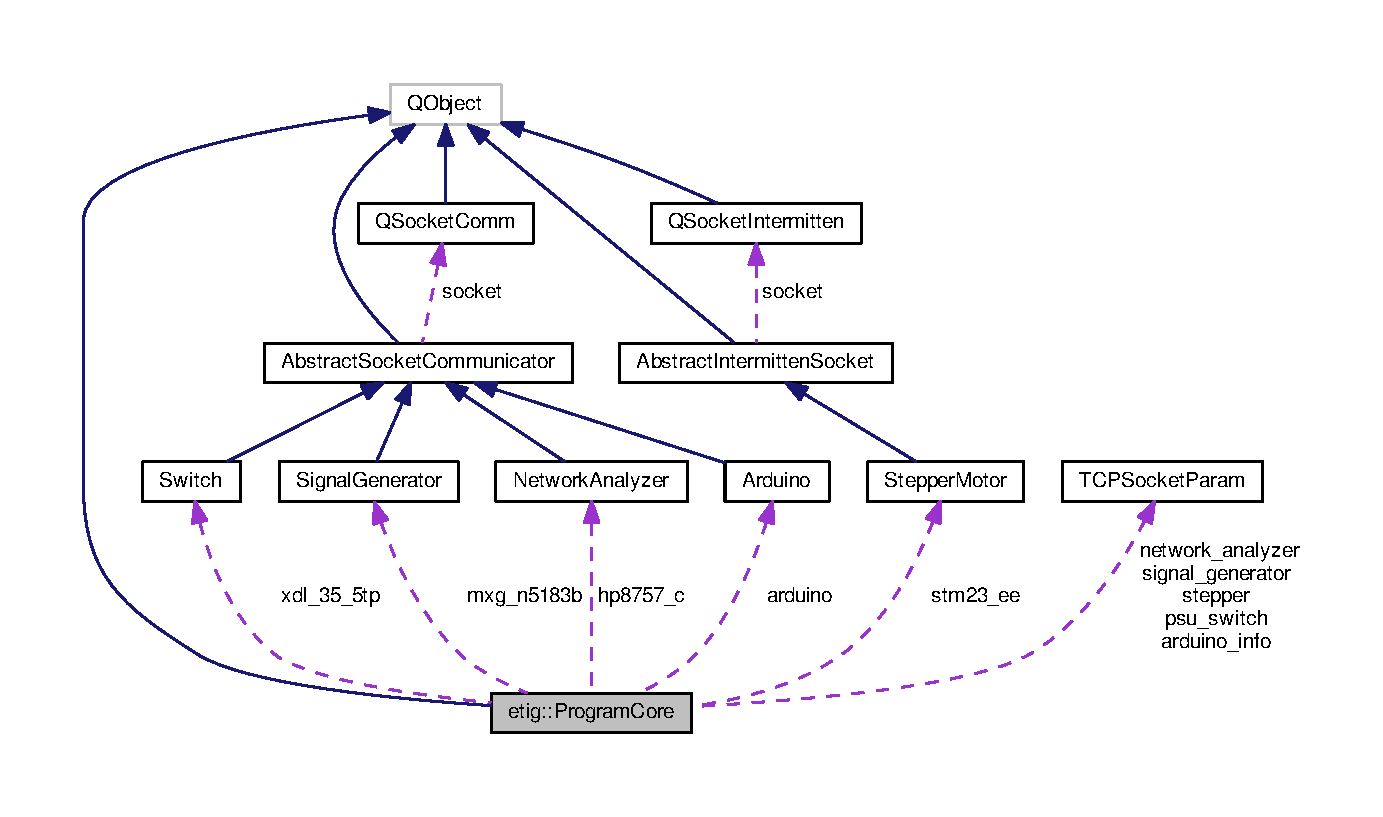
\includegraphics[width=350pt]{classetig_1_1_program_core__coll__graph}
\end{center}
\end{figure}
\subsection*{Public Member Functions}
\begin{DoxyCompactItemize}
\item 
{\bfseries Program\+Core} (Q\+Object $\ast$parent=0)\hypertarget{classetig_1_1_program_core_a0f0556682ac02580cf51c679af994183}{}\label{classetig_1_1_program_core_a0f0556682ac02580cf51c679af994183}

\item 
void {\bfseries Retract\+Cavity} ()\hypertarget{classetig_1_1_program_core_a254509de2bfaf73b4dfa9442b55ea394}{}\label{classetig_1_1_program_core_a254509de2bfaf73b4dfa9442b55ea394}

\item 
void {\bfseries Rapid\+Traverse} ()\hypertarget{classetig_1_1_program_core_a6a1be8a5e7abf50fdb4a896137bc505a}{}\label{classetig_1_1_program_core_a6a1be8a5e7abf50fdb4a896137bc505a}

\item 
void {\bfseries Prequel\+Transmission} ()\hypertarget{classetig_1_1_program_core_a1fab0d46ede7eb2304e586d9375732f7}{}\label{classetig_1_1_program_core_a1fab0d46ede7eb2304e586d9375732f7}

\item 
void {\bfseries Prequel\+Reflection} ()\hypertarget{classetig_1_1_program_core_aeb11b8b520d4f0224713dbd5d983d636}{}\label{classetig_1_1_program_core_aeb11b8b520d4f0224713dbd5d983d636}

\item 
void {\bfseries Next\+Iteration} ()\hypertarget{classetig_1_1_program_core_a34d16d1c70c2d45a1fcbad1902c9de21}{}\label{classetig_1_1_program_core_a34d16d1c70c2d45a1fcbad1902c9de21}

\item 
void {\bfseries Jitter} ()\hypertarget{classetig_1_1_program_core_a069a482c22c525a4081225ba3bec2c0a}{}\label{classetig_1_1_program_core_a069a482c22c525a4081225ba3bec2c0a}

\end{DoxyCompactItemize}
\subsection*{Protected Member Functions}
\begin{DoxyCompactItemize}
\item 
void {\bfseries Move\+To\+B\+G\+Subtraction\+Length} ()\hypertarget{classetig_1_1_program_core_a3a405439926758a6da7658180659cfec}{}\label{classetig_1_1_program_core_a3a405439926758a6da7658180659cfec}

\item 
void {\bfseries Move\+To\+Start\+Length} ()\hypertarget{classetig_1_1_program_core_a4f2760f926277d8829d3f65cbd95260c}{}\label{classetig_1_1_program_core_a4f2760f926277d8829d3f65cbd95260c}

\item 
void {\bfseries Move\+To\+End\+Length} ()\hypertarget{classetig_1_1_program_core_a11429f35f59e9540b886163c6a7eb211}{}\label{classetig_1_1_program_core_a11429f35f59e9540b886163c6a7eb211}

\end{DoxyCompactItemize}
\subsection*{Protected Attributes}
\begin{DoxyCompactItemize}
\item 
const std\+::string {\bfseries save\+\_\+file\+\_\+path} = \char`\"{}/home/admx/Electric\+\_\+\+Tiger\+\_\+\+Data/\char`\"{}\hypertarget{classetig_1_1_program_core_a676ae3389038bf3fd3ba72d25c91ca14}{}\label{classetig_1_1_program_core_a676ae3389038bf3fd3ba72d25c91ca14}

\item 
const double {\bfseries length\+\_\+of\+\_\+tune} = 2.\+0\hypertarget{classetig_1_1_program_core_a2e5f6bcfde100f8b02bc27759bca2634}{}\label{classetig_1_1_program_core_a2e5f6bcfde100f8b02bc27759bca2634}

\item 
const double {\bfseries revs\+\_\+per\+\_\+iterations} = 1\hypertarget{classetig_1_1_program_core_aebaed1df58743c5d2153e24d130d0a8c}{}\label{classetig_1_1_program_core_aebaed1df58743c5d2153e24d130d0a8c}

\item 
const double {\bfseries start\+\_\+length} = 7.\+0\hypertarget{classetig_1_1_program_core_af9378cd76eb6a08a0f4ee68e7e1e38d2}{}\label{classetig_1_1_program_core_af9378cd76eb6a08a0f4ee68e7e1e38d2}

\item 
const double {\bfseries background\+\_\+scan\+\_\+length} = 5.\+0\hypertarget{classetig_1_1_program_core_a9df4bede1a3ce203653cf350a2aebe0c}{}\label{classetig_1_1_program_core_a9df4bede1a3ce203653cf350a2aebe0c}

\item 
const double {\bfseries nwa\+\_\+span\+\_\+\+M\+Hz} = 400.\+0\hypertarget{classetig_1_1_program_core_aae6510cbce708f827a8e0a68f35faddc}{}\label{classetig_1_1_program_core_aae6510cbce708f827a8e0a68f35faddc}

\item 
const uint {\bfseries nwa\+\_\+points} = 401\hypertarget{classetig_1_1_program_core_ad7add3a027aa2b2658b207ada1b900b7}{}\label{classetig_1_1_program_core_ad7add3a027aa2b2658b207ada1b900b7}

\item 
const double {\bfseries nwa\+\_\+power\+\_\+d\+Bm} = -\/15.\+0\hypertarget{classetig_1_1_program_core_a37f048a230fc7e4c9720b8b283acec72}{}\label{classetig_1_1_program_core_a37f048a230fc7e4c9720b8b283acec72}

\item 
const double {\bfseries signal\+\_\+generator\+\_\+power\+\_\+d\+Bm} = 15.\+0\hypertarget{classetig_1_1_program_core_ae75519ef4954fa2c1574428743e28143}{}\label{classetig_1_1_program_core_ae75519ef4954fa2c1574428743e28143}

\item 
const double {\bfseries freq\+\_\+window\+\_\+\+M\+Hz} = 100.\+0\hypertarget{classetig_1_1_program_core_a6f2bb8b5e0302f06768cf0dcc4ec144b}{}\label{classetig_1_1_program_core_a6f2bb8b5e0302f06768cf0dcc4ec144b}

\item 
const double {\bfseries digitizer\+\_\+rate\+\_\+\+M\+Hz} = 180.\+0\hypertarget{classetig_1_1_program_core_aa7f5ff1910379a1a8289b7bf90a9d67e}{}\label{classetig_1_1_program_core_aa7f5ff1910379a1a8289b7bf90a9d67e}

\item 
const double {\bfseries na\+\_\+min\+\_\+freq} = 3000.\+0\hypertarget{classetig_1_1_program_core_a67d8315993116e9e18d86b81b4a13cf8}{}\label{classetig_1_1_program_core_a67d8315993116e9e18d86b81b4a13cf8}

\item 
const double {\bfseries na\+\_\+max\+\_\+freq} = 4600.\+0\hypertarget{classetig_1_1_program_core_a233d0a5af3b5a9855497e856c8728fac}{}\label{classetig_1_1_program_core_a233d0a5af3b5a9855497e856c8728fac}

\item 
const uint {\bfseries num\+\_\+averages} = 10000\hypertarget{classetig_1_1_program_core_a45e70a7c9fda697e2e9882614647a67e}{}\label{classetig_1_1_program_core_a45e70a7c9fda697e2e9882614647a67e}

\item 
uint {\bfseries rebin\+\_\+size} = 0\hypertarget{classetig_1_1_program_core_aa451c512891ac93ba9f07ed4474e558f}{}\label{classetig_1_1_program_core_aa451c512891ac93ba9f07ed4474e558f}

\item 
const \hyperlink{struct_t_c_p_socket_param}{T\+C\+P\+Socket\+Param} {\bfseries psu\+\_\+switch} = \hyperlink{struct_t_c_p_socket_param}{T\+C\+P\+Socket\+Param}( \char`\"{}Switch\char`\"{}, \char`\"{}10.\+95.\+100.\+174\char`\"{}, 9221 )\hypertarget{classetig_1_1_program_core_a0e2454403a85b97801f772e720b01631}{}\label{classetig_1_1_program_core_a0e2454403a85b97801f772e720b01631}

\item 
const \hyperlink{struct_t_c_p_socket_param}{T\+C\+P\+Socket\+Param} {\bfseries network\+\_\+analyzer} = \hyperlink{struct_t_c_p_socket_param}{T\+C\+P\+Socket\+Param}( \char`\"{}Network\+Analyzer\char`\"{}, \char`\"{}10.\+95.\+100.\+176\char`\"{}, 1234 )\hypertarget{classetig_1_1_program_core_ab730e120b7ea8d72101d4002d816e8ec}{}\label{classetig_1_1_program_core_ab730e120b7ea8d72101d4002d816e8ec}

\item 
const \hyperlink{struct_t_c_p_socket_param}{T\+C\+P\+Socket\+Param} {\bfseries stepper} = \hyperlink{struct_t_c_p_socket_param}{T\+C\+P\+Socket\+Param}( \char`\"{}Stepper\char`\"{}, \char`\"{}10.\+95.\+100.\+177\char`\"{}, 7776 )\hypertarget{classetig_1_1_program_core_a4b8a04ab5747b0f9a247dadd7118b654}{}\label{classetig_1_1_program_core_a4b8a04ab5747b0f9a247dadd7118b654}

\item 
const \hyperlink{struct_t_c_p_socket_param}{T\+C\+P\+Socket\+Param} {\bfseries signal\+\_\+generator} = \hyperlink{struct_t_c_p_socket_param}{T\+C\+P\+Socket\+Param}( \char`\"{}Signal\+Generator\char`\"{}, \char`\"{}10.\+95.\+100.\+175\char`\"{}, 5025 )\hypertarget{classetig_1_1_program_core_a9ae804b8a25e4ad6fdc3a2fc023667a0}{}\label{classetig_1_1_program_core_a9ae804b8a25e4ad6fdc3a2fc023667a0}

\item 
const \hyperlink{struct_t_c_p_socket_param}{T\+C\+P\+Socket\+Param} {\bfseries arduino\+\_\+info} = \hyperlink{struct_t_c_p_socket_param}{T\+C\+P\+Socket\+Param}( \char`\"{}Arduino\char`\"{}, \char`\"{}10.\+95.\+100.\+173\char`\"{}, 23 )\hypertarget{classetig_1_1_program_core_a071fd67790cc4f2ea909f33ebe19710c}{}\label{classetig_1_1_program_core_a071fd67790cc4f2ea909f33ebe19710c}

\item 
std\+::shared\+\_\+ptr$<$ A\+T\+S9462\+Engine $>$ {\bfseries ats9462}\hypertarget{classetig_1_1_program_core_a4ec687ca2ad049330abe582dc98e0155}{}\label{classetig_1_1_program_core_a4ec687ca2ad049330abe582dc98e0155}

\item 
\hyperlink{class_arduino}{Arduino} $\ast$ {\bfseries arduino}\hypertarget{classetig_1_1_program_core_af68538ad2f740c504af9f02c74f2e899}{}\label{classetig_1_1_program_core_af68538ad2f740c504af9f02c74f2e899}

\item 
\hyperlink{class_network_analyzer}{Network\+Analyzer} $\ast$ {\bfseries hp8757\+\_\+c}\hypertarget{classetig_1_1_program_core_a97b51dfcdeb19a3e1f7795366f208fb8}{}\label{classetig_1_1_program_core_a97b51dfcdeb19a3e1f7795366f208fb8}

\item 
\hyperlink{class_signal_generator}{Signal\+Generator} $\ast$ {\bfseries mxg\+\_\+n5183b}\hypertarget{classetig_1_1_program_core_aa2c7133f1c63bcbbffe4e7624b643752}{}\label{classetig_1_1_program_core_aa2c7133f1c63bcbbffe4e7624b643752}

\item 
\hyperlink{class_stepper_motor}{Stepper\+Motor} $\ast$ {\bfseries stm23\+\_\+ee}\hypertarget{classetig_1_1_program_core_ae54ac562120bf6c622f08cccd1eb2885}{}\label{classetig_1_1_program_core_ae54ac562120bf6c622f08cccd1eb2885}

\item 
\hyperlink{class_switch}{Switch} $\ast$ {\bfseries xdl\+\_\+35\+\_\+5tp}\hypertarget{classetig_1_1_program_core_afd776ceb26508e55631f6bc20de623fe}{}\label{classetig_1_1_program_core_afd776ceb26508e55631f6bc20de623fe}

\item 
double {\bfseries number\+\_\+of\+\_\+iterations} = 0.\+0\hypertarget{classetig_1_1_program_core_a4f29550ef3feda2f0818009f977e4db5}{}\label{classetig_1_1_program_core_a4f29550ef3feda2f0818009f977e4db5}

\item 
uint {\bfseries iteration} = 0\hypertarget{classetig_1_1_program_core_a2b9431f383533162e5dad9881e3bd2ac}{}\label{classetig_1_1_program_core_a2b9431f383533162e5dad9881e3bd2ac}

\end{DoxyCompactItemize}


The documentation for this class was generated from the following files\+:\begin{DoxyCompactItemize}
\item 
/home/bephillips2/\+Qt-\/\+Projects/\+Electric\+\_\+\+Tiger\+\_\+\+D\+A\+Q/\+Program/\+Program\+Core/programcore.\+h\item 
/home/bephillips2/\+Qt-\/\+Projects/\+Electric\+\_\+\+Tiger\+\_\+\+D\+A\+Q/\+Program/\+Program\+Core/programcore.\+cpp\end{DoxyCompactItemize}

\hypertarget{classetig_1_1_program_frame}{}\section{etig\+:\+:Program\+Frame Class Reference}
\label{classetig_1_1_program_frame}\index{etig\+::\+Program\+Frame@{etig\+::\+Program\+Frame}}


Inheritance diagram for etig\+:\+:Program\+Frame\+:\nopagebreak
\begin{figure}[H]
\begin{center}
\leavevmode
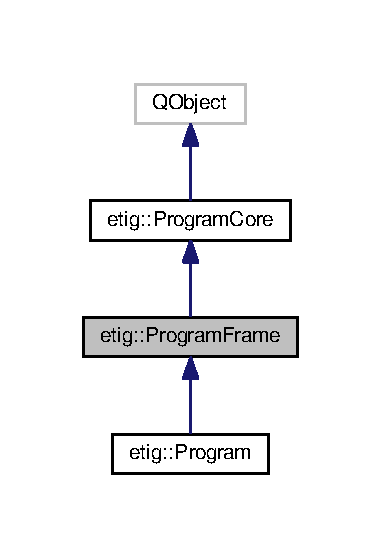
\includegraphics[width=183pt]{classetig_1_1_program_frame__inherit__graph}
\end{center}
\end{figure}


Collaboration diagram for etig\+:\+:Program\+Frame\+:\nopagebreak
\begin{figure}[H]
\begin{center}
\leavevmode
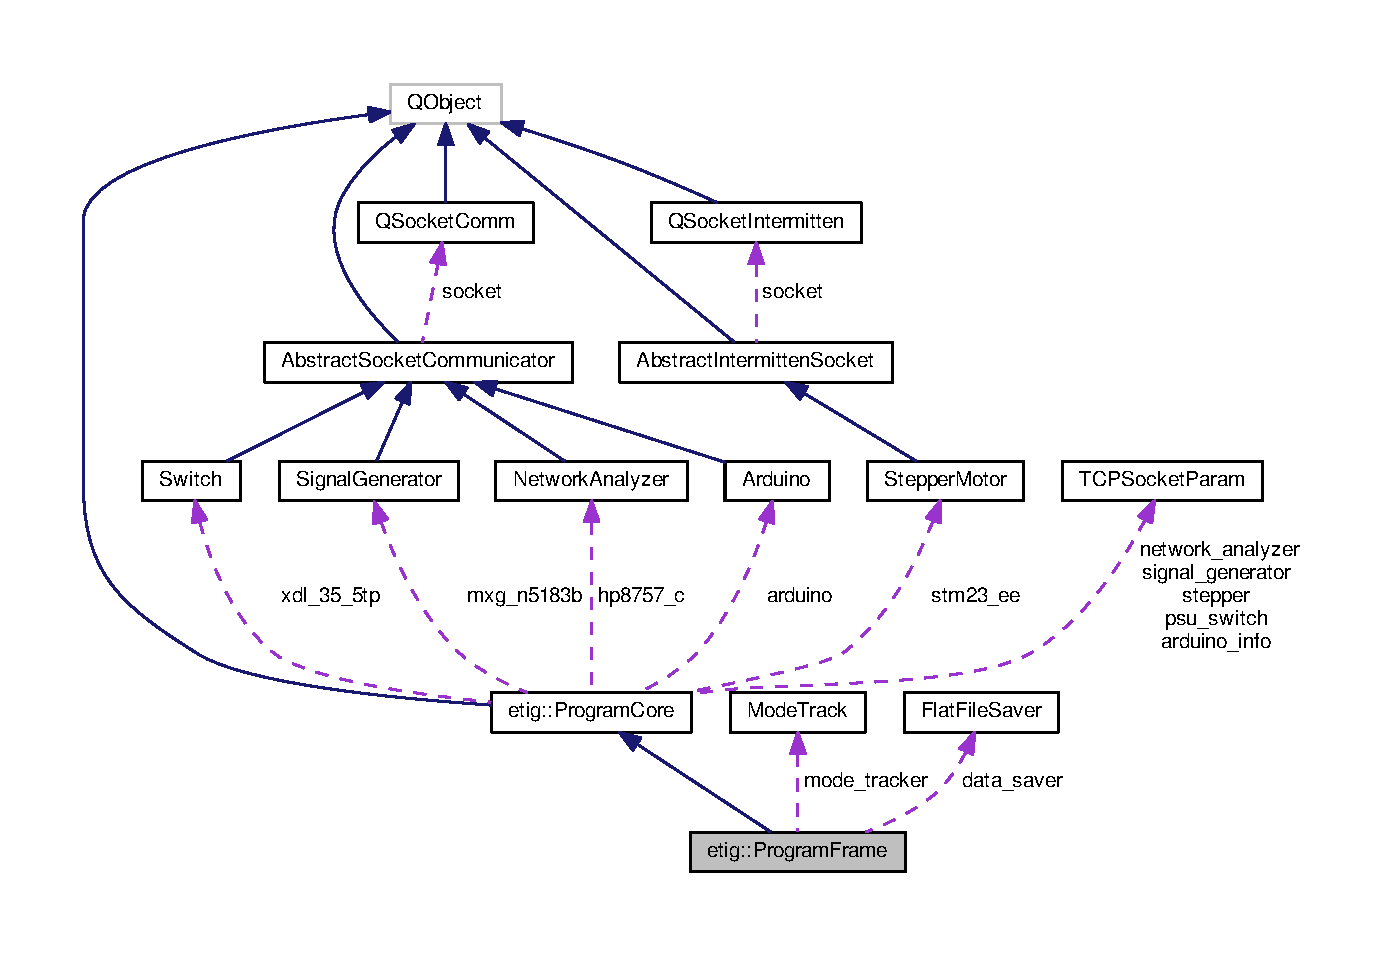
\includegraphics[width=350pt]{classetig_1_1_program_frame__coll__graph}
\end{center}
\end{figure}
\subsection*{Signals}
\begin{DoxyCompactItemize}
\item 
void {\bfseries Update\+NA} (std\+::vector$<$ double $>$ na\+\_\+data, double na\+\_\+span)\hypertarget{classetig_1_1_program_frame_a824d1e9e44d999d4a5a587b3f9613fa8}{}\label{classetig_1_1_program_frame_a824d1e9e44d999d4a5a587b3f9613fa8}

\item 
void {\bfseries Update\+Spec} (std\+::vector$<$ float $>$ spec\+\_\+data, uint digi\+\_\+rate)\hypertarget{classetig_1_1_program_frame_ad9248e8416130ac077fd4d765382a093}{}\label{classetig_1_1_program_frame_ad9248e8416130ac077fd4d765382a093}

\item 
void {\bfseries To\+Transmission} ()\hypertarget{classetig_1_1_program_frame_ae39d5e3b652f9725e31d8969be4e108b}{}\label{classetig_1_1_program_frame_ae39d5e3b652f9725e31d8969be4e108b}

\item 
void {\bfseries To\+Reflection} ()\hypertarget{classetig_1_1_program_frame_a391fa1884342324998b4a6b12d009db4}{}\label{classetig_1_1_program_frame_a391fa1884342324998b4a6b12d009db4}

\item 
void {\bfseries Output\+To\+Digitizer} ()\hypertarget{classetig_1_1_program_frame_a5a6803a49009713800cab9b931326dc6}{}\label{classetig_1_1_program_frame_a5a6803a49009713800cab9b931326dc6}

\item 
void {\bfseries Output\+To\+NA} ()\hypertarget{classetig_1_1_program_frame_a47f1db16a6ca7f0a2c95c94f11d89128}{}\label{classetig_1_1_program_frame_a47f1db16a6ca7f0a2c95c94f11d89128}

\item 
void {\bfseries Iteration} (uint iter)\hypertarget{classetig_1_1_program_frame_a35e9a4ff69d563cef9f43bf737a17880}{}\label{classetig_1_1_program_frame_a35e9a4ff69d563cef9f43bf737a17880}

\item 
void {\bfseries Cavity\+Length} (double length)\hypertarget{classetig_1_1_program_frame_a6e05071a1bf4649e1ec1082581a451c7}{}\label{classetig_1_1_program_frame_a6e05071a1bf4649e1ec1082581a451c7}

\item 
void {\bfseries L\+O\+Frequency} (double lo\+\_\+freq)\hypertarget{classetig_1_1_program_frame_a1209484236960c92deea722171b2a783}{}\label{classetig_1_1_program_frame_a1209484236960c92deea722171b2a783}

\end{DoxyCompactItemize}
\subsection*{Public Member Functions}
\begin{DoxyCompactItemize}
\item 
{\bfseries Program\+Frame} (Q\+Object $\ast$parent)\hypertarget{classetig_1_1_program_frame_a69871d3d3ee8ca09985eea46ab2df1de}{}\label{classetig_1_1_program_frame_a69871d3d3ee8ca09985eea46ab2df1de}

\item 
void {\bfseries Prequel} ()\hypertarget{classetig_1_1_program_frame_a2da29d05f66287788c42ba5ba28e5b9b}{}\label{classetig_1_1_program_frame_a2da29d05f66287788c42ba5ba28e5b9b}

\item 
void {\bfseries Shift\+Frequency\+Window} (double center\+\_\+frequency)\hypertarget{classetig_1_1_program_frame_a4b5a587570c2dbad42af57575b395bbb}{}\label{classetig_1_1_program_frame_a4b5a587570c2dbad42af57575b395bbb}

\item 
void {\bfseries Set\+Background} ()\hypertarget{classetig_1_1_program_frame_af41867166a0bc9c5f488107595fedb13}{}\label{classetig_1_1_program_frame_af41867166a0bc9c5f488107595fedb13}

\item 
void {\bfseries Establish\+Bin\+Size} ()\hypertarget{classetig_1_1_program_frame_a04305476dafab8c721d7b8eb41549239}{}\label{classetig_1_1_program_frame_a04305476dafab8c721d7b8eb41549239}

\item 
double {\bfseries Find\+Minima\+Peak} (data\+\_\+list formatted\+\_\+points)\hypertarget{classetig_1_1_program_frame_a72eedcd0f69f164ab687f8244a3ec530}{}\label{classetig_1_1_program_frame_a72eedcd0f69f164ab687f8244a3ec530}

\end{DoxyCompactItemize}
\subsection*{Protected Member Functions}
\begin{DoxyCompactItemize}
\item 
data\+\_\+list {\bfseries power\+\_\+to\+\_\+data\+\_\+list} (std\+::vector$<$ float $>$ power\+\_\+list, float min\+\_\+freq, float max\+\_\+freq)\hypertarget{classetig_1_1_program_frame_a1e970cac4d1173733d27cd8f3bbaf2fb}{}\label{classetig_1_1_program_frame_a1e970cac4d1173733d27cd8f3bbaf2fb}

\item 
data\+\_\+list {\bfseries power\+\_\+to\+\_\+data\+\_\+list} (std\+::vector$<$ double $>$ power\+\_\+list, double min\+\_\+freq, double max\+\_\+freq)\hypertarget{classetig_1_1_program_frame_add41bacb448ca38d6923a2a31b71a497}{}\label{classetig_1_1_program_frame_add41bacb448ca38d6923a2a31b71a497}

\item 
{\footnotesize template$<$typename T $>$ }\\std\+::vector$<$ T $>$ {\bfseries data\+\_\+list\+\_\+to\+\_\+power} (std\+::vector$<$ \hyperlink{structdata__triple}{data\+\_\+triple}$<$ T $>$ $>$ data)\hypertarget{classetig_1_1_program_frame_aacd3bf2aed00a0ae7d6c6c99348a7f6d}{}\label{classetig_1_1_program_frame_aacd3bf2aed00a0ae7d6c6c99348a7f6d}

\item 
double {\bfseries Check\+Peak} (double possible\+\_\+mode\+\_\+position)\hypertarget{classetig_1_1_program_frame_a6bd23443debb7304d18de76d7550c8dd}{}\label{classetig_1_1_program_frame_a6bd23443debb7304d18de76d7550c8dd}

\item 
std\+::string {\bfseries Build\+Header} ()\hypertarget{classetig_1_1_program_frame_a74ffbb16b183e7b3d485183f41501e75}{}\label{classetig_1_1_program_frame_a74ffbb16b183e7b3d485183f41501e75}

\end{DoxyCompactItemize}
\subsection*{Protected Attributes}
\begin{DoxyCompactItemize}
\item 
\hyperlink{class_mode_track}{Mode\+Track} {\bfseries mode\+\_\+tracker}\hypertarget{classetig_1_1_program_frame_aea8eb7ef9e89cb2647a43e29bde12c98}{}\label{classetig_1_1_program_frame_aea8eb7ef9e89cb2647a43e29bde12c98}

\item 
\hyperlink{class_flat_file_saver}{Flat\+File\+Saver} {\bfseries data\+\_\+saver} \{ save\+\_\+file\+\_\+path \}\hypertarget{classetig_1_1_program_frame_a4338418648f4eff77b8fd7666e1938ea}{}\label{classetig_1_1_program_frame_a4338418648f4eff77b8fd7666e1938ea}

\end{DoxyCompactItemize}


The documentation for this class was generated from the following files\+:\begin{DoxyCompactItemize}
\item 
/home/bephillips2/\+Qt-\/\+Projects/\+Electric\+\_\+\+Tiger\+\_\+\+D\+A\+Q/\+Program/\+Program\+Frame/programframe.\+h\item 
/home/bephillips2/\+Qt-\/\+Projects/\+Electric\+\_\+\+Tiger\+\_\+\+D\+A\+Q/\+Program/\+Program\+Frame/programframe.\+cpp\end{DoxyCompactItemize}

\hypertarget{class_q_socket_comm}{}\section{Q\+Socket\+Comm Class Reference}
\label{class_q_socket_comm}\index{Q\+Socket\+Comm@{Q\+Socket\+Comm}}


Inheritance diagram for Q\+Socket\+Comm\+:\nopagebreak
\begin{figure}[H]
\begin{center}
\leavevmode
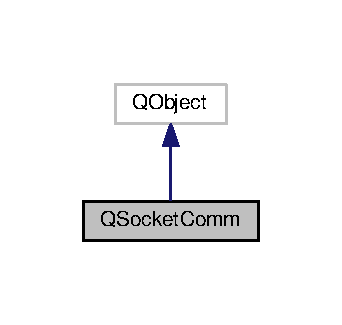
\includegraphics[width=164pt]{class_q_socket_comm__inherit__graph}
\end{center}
\end{figure}


Collaboration diagram for Q\+Socket\+Comm\+:\nopagebreak
\begin{figure}[H]
\begin{center}
\leavevmode
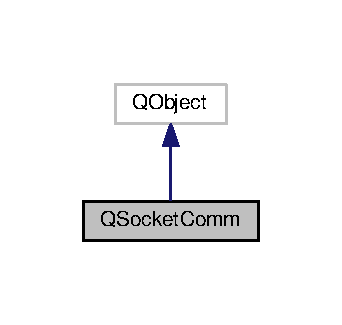
\includegraphics[width=164pt]{class_q_socket_comm__coll__graph}
\end{center}
\end{figure}
\subsection*{Public Member Functions}
\begin{DoxyCompactItemize}
\item 
{\bfseries Q\+Socket\+Comm} (std\+::string host\+\_\+name, uint port\+\_\+number, Q\+Object $\ast$parent=0)\hypertarget{class_q_socket_comm_afe66e31a1196650b60883380ae7dd141}{}\label{class_q_socket_comm_afe66e31a1196650b60883380ae7dd141}

\item 
void {\bfseries Send} (std\+::string command, std\+::string terminator=\char`\"{}\textbackslash{}n\char`\"{})\hypertarget{class_q_socket_comm_a6642ec94f586abdb30dfe0c0532b3bca}{}\label{class_q_socket_comm_a6642ec94f586abdb30dfe0c0532b3bca}

\item 
void {\bfseries Send\+Scl} (std\+::string command)\hypertarget{class_q_socket_comm_a900132260caef9b4e8b959350a5dfd06}{}\label{class_q_socket_comm_a900132260caef9b4e8b959350a5dfd06}

\item 
std\+::string {\bfseries Receive} ()\hypertarget{class_q_socket_comm_af3bd1b626085af405bd27dacf54950e1}{}\label{class_q_socket_comm_af3bd1b626085af405bd27dacf54950e1}

\item 
std\+::string {\bfseries Receive\+Safe} ()\hypertarget{class_q_socket_comm_a7e695332f9bca48a446bf446bd59acda}{}\label{class_q_socket_comm_a7e695332f9bca48a446bf446bd59acda}

\end{DoxyCompactItemize}


The documentation for this class was generated from the following files\+:\begin{DoxyCompactItemize}
\item 
/home/bephillips2/\+Qt-\/\+Projects/\+Electric\+\_\+\+Tiger\+\_\+\+D\+A\+Q/\+Socket\+Communicators/\+Socket\+Comm/q\+\_\+socket\+\_\+comm.\+h\item 
/home/bephillips2/\+Qt-\/\+Projects/\+Electric\+\_\+\+Tiger\+\_\+\+D\+A\+Q/\+Socket\+Communicators/\+Socket\+Comm/q\+\_\+socket\+\_\+comm.\+cpp\end{DoxyCompactItemize}

\hypertarget{class_q_socket_intermitten}{}\section{Q\+Socket\+Intermitten Class Reference}
\label{class_q_socket_intermitten}\index{Q\+Socket\+Intermitten@{Q\+Socket\+Intermitten}}


Inheritance diagram for Q\+Socket\+Intermitten\+:\nopagebreak
\begin{figure}[H]
\begin{center}
\leavevmode
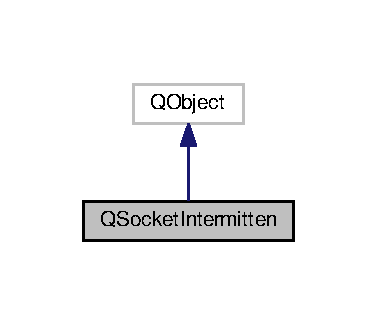
\includegraphics[width=181pt]{class_q_socket_intermitten__inherit__graph}
\end{center}
\end{figure}


Collaboration diagram for Q\+Socket\+Intermitten\+:\nopagebreak
\begin{figure}[H]
\begin{center}
\leavevmode
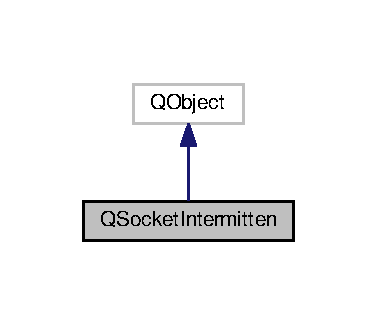
\includegraphics[width=181pt]{class_q_socket_intermitten__coll__graph}
\end{center}
\end{figure}
\subsection*{Public Member Functions}
\begin{DoxyCompactItemize}
\item 
{\bfseries Q\+Socket\+Intermitten} (std\+::string host\+\_\+name, uint port\+\_\+number, Q\+Object $\ast$parent=0)\hypertarget{class_q_socket_intermitten_a10efaac40d71a525574fe238ebf0db74}{}\label{class_q_socket_intermitten_a10efaac40d71a525574fe238ebf0db74}

\item 
void {\bfseries Open\+Connection} ()\hypertarget{class_q_socket_intermitten_a01b636438109d46a2135f67dbb5446aa}{}\label{class_q_socket_intermitten_a01b636438109d46a2135f67dbb5446aa}

\item 
void {\bfseries Close\+Connection} ()\hypertarget{class_q_socket_intermitten_abecdd03c978b32edf1e464bb91ce5314}{}\label{class_q_socket_intermitten_abecdd03c978b32edf1e464bb91ce5314}

\item 
void {\bfseries Send} (std\+::string command, std\+::string terminator=\char`\"{}\textbackslash{}n\char`\"{})\hypertarget{class_q_socket_intermitten_a989c6bb818303c7a3119025d30c4aff6}{}\label{class_q_socket_intermitten_a989c6bb818303c7a3119025d30c4aff6}

\item 
void {\bfseries Send\+Scl} (std\+::string command)\hypertarget{class_q_socket_intermitten_a1c290c38ffec48bf30f93ad40bc82aaa}{}\label{class_q_socket_intermitten_a1c290c38ffec48bf30f93ad40bc82aaa}

\item 
std\+::string {\bfseries Receive} ()\hypertarget{class_q_socket_intermitten_a40414faabe73f8787499c27c34794aea}{}\label{class_q_socket_intermitten_a40414faabe73f8787499c27c34794aea}

\item 
std\+::string {\bfseries Receive\+Safe} ()\hypertarget{class_q_socket_intermitten_a05db0fd6ead8cd00f486d9e7f1a48caa}{}\label{class_q_socket_intermitten_a05db0fd6ead8cd00f486d9e7f1a48caa}

\end{DoxyCompactItemize}


The documentation for this class was generated from the following files\+:\begin{DoxyCompactItemize}
\item 
/home/bephillips2/\+Qt-\/\+Projects/\+Electric\+\_\+\+Tiger\+\_\+\+D\+A\+Q/\+Socket\+Communicators/\+Socket\+Comm/qsocketintermitten.\+h\item 
/home/bephillips2/\+Qt-\/\+Projects/\+Electric\+\_\+\+Tiger\+\_\+\+D\+A\+Q/\+Socket\+Communicators/\+Socket\+Comm/qsocketintermitten.\+cpp\end{DoxyCompactItemize}

\hypertarget{structetig_1_1_rebin}{}\section{etig\+:\+:Rebin$<$ T $>$ Struct Template Reference}
\label{structetig_1_1_rebin}\index{etig\+::\+Rebin$<$ T $>$@{etig\+::\+Rebin$<$ T $>$}}
\subsection*{Public Member Functions}
\begin{DoxyCompactItemize}
\item 
void \hyperlink{structetig_1_1_rebin_a35e4d74f8a7246fea553ced3d36dd2e2}{operator()} (const std\+::vector$<$ T $>$ \&time\+\_\+series, T f\+\_\+res, T time\+\_\+int)
\begin{DoxyCompactList}\small\item\em operator () \end{DoxyCompactList}\item 
void \hyperlink{structetig_1_1_rebin_a19fa21958e651977f7d2664bb6f71fd3}{operator()} (const std\+::vector$<$ T $>$ \&time\+\_\+series, uint overbin\+\_\+size)
\begin{DoxyCompactList}\small\item\em operator () \end{DoxyCompactList}\item 
std\+::vector$<$ T $>$ {\bfseries Rebinned\+Signal} ()\hypertarget{structetig_1_1_rebin_afa8fd00980940055279a2c35eba4b43d}{}\label{structetig_1_1_rebin_afa8fd00980940055279a2c35eba4b43d}

\item 
uint {\bfseries Rebin\+Size} ()\hypertarget{structetig_1_1_rebin_a90e8b55c1201f4c958cdf0c46d99e364}{}\label{structetig_1_1_rebin_a90e8b55c1201f4c958cdf0c46d99e364}

\end{DoxyCompactItemize}


\subsection{Member Function Documentation}
\index{etig\+::\+Rebin@{etig\+::\+Rebin}!operator()@{operator()}}
\index{operator()@{operator()}!etig\+::\+Rebin@{etig\+::\+Rebin}}
\subsubsection[{\texorpdfstring{operator()(const std\+::vector$<$ T $>$ \&time\+\_\+series, T f\+\_\+res, T time\+\_\+int)}{operator()(const std::vector< T > &time_series, T f_res, T time_int)}}]{\setlength{\rightskip}{0pt plus 5cm}template$<$typename T$>$ void {\bf etig\+::\+Rebin}$<$ T $>$\+::operator() (
\begin{DoxyParamCaption}
\item[{const std\+::vector$<$ T $>$ \&}]{time\+\_\+series, }
\item[{T}]{f\+\_\+res, }
\item[{T}]{time\+\_\+int}
\end{DoxyParamCaption}
)\hspace{0.3cm}{\ttfamily [inline]}}\hypertarget{structetig_1_1_rebin_a35e4d74f8a7246fea553ced3d36dd2e2}{}\label{structetig_1_1_rebin_a35e4d74f8a7246fea553ced3d36dd2e2}


operator () 


\begin{DoxyParams}{Parameters}
{\em time\+\_\+series} & The raw power signal that needs to be re-\/binned\\
\hline
{\em f\+\_\+res} & Center frequency of the current mode ( in M\+Hz )\\
\hline
{\em time\+\_\+int} & Total time that time\+\_\+series was collected over ( in seconds ) \\
\hline
\end{DoxyParams}
\index{etig\+::\+Rebin@{etig\+::\+Rebin}!operator()@{operator()}}
\index{operator()@{operator()}!etig\+::\+Rebin@{etig\+::\+Rebin}}
\subsubsection[{\texorpdfstring{operator()(const std\+::vector$<$ T $>$ \&time\+\_\+series, uint overbin\+\_\+size)}{operator()(const std::vector< T > &time_series, uint overbin_size)}}]{\setlength{\rightskip}{0pt plus 5cm}template$<$typename T$>$ void {\bf etig\+::\+Rebin}$<$ T $>$\+::operator() (
\begin{DoxyParamCaption}
\item[{const std\+::vector$<$ T $>$ \&}]{time\+\_\+series, }
\item[{uint}]{overbin\+\_\+size}
\end{DoxyParamCaption}
)\hspace{0.3cm}{\ttfamily [inline]}}\hypertarget{structetig_1_1_rebin_a19fa21958e651977f7d2664bb6f71fd3}{}\label{structetig_1_1_rebin_a19fa21958e651977f7d2664bb6f71fd3}


operator () 


\begin{DoxyParams}{Parameters}
{\em time\+\_\+series} & The raw power signal that needs to be re-\/binned\\
\hline
{\em overbin\+\_\+size} & Number of elements that should be averaged into a single bin. \\
\hline
\end{DoxyParams}


The documentation for this struct was generated from the following file\+:\begin{DoxyCompactItemize}
\item 
/home/bephillips2/\+Qt-\/\+Projects/\+Electric\+\_\+\+Tiger\+\_\+\+D\+A\+Q/\+Algorithm/algorithm.\+h\end{DoxyCompactItemize}

\hypertarget{struct_retrieve_val}{}\section{Retrieve\+Val Struct Reference}
\label{struct_retrieve_val}\index{Retrieve\+Val@{Retrieve\+Val}}
\subsection*{Public Member Functions}
\begin{DoxyCompactItemize}
\item 
{\footnotesize template$<$typename T $>$ }\\T\+::first\+\_\+type {\bfseries operator()} (T key\+Value\+Pair) const \hypertarget{struct_retrieve_val_a497045c23da008812919a69049998b1e}{}\label{struct_retrieve_val_a497045c23da008812919a69049998b1e}

\end{DoxyCompactItemize}


The documentation for this struct was generated from the following file\+:\begin{DoxyCompactItemize}
\item 
/home/bephillips2/\+Qt-\/\+Projects/\+Electric\+\_\+\+Tiger\+\_\+\+D\+A\+Q/\+Mode\+Tracker/modetrack.\+cpp\end{DoxyCompactItemize}

\hypertarget{class_right_click_menu}{}\section{Right\+Click\+Menu Class Reference}
\label{class_right_click_menu}\index{Right\+Click\+Menu@{Right\+Click\+Menu}}


Inheritance diagram for Right\+Click\+Menu\+:\nopagebreak
\begin{figure}[H]
\begin{center}
\leavevmode
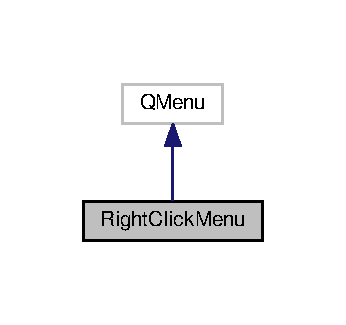
\includegraphics[width=166pt]{class_right_click_menu__inherit__graph}
\end{center}
\end{figure}


Collaboration diagram for Right\+Click\+Menu\+:\nopagebreak
\begin{figure}[H]
\begin{center}
\leavevmode
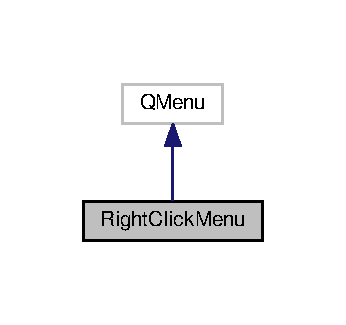
\includegraphics[width=166pt]{class_right_click_menu__coll__graph}
\end{center}
\end{figure}
\subsection*{Signals}
\begin{DoxyCompactItemize}
\item 
void {\bfseries Scaling} ()\hypertarget{class_right_click_menu_a5607dbc6616a76b431cd77ce47d6a1ee}{}\label{class_right_click_menu_a5607dbc6616a76b431cd77ce47d6a1ee}

\end{DoxyCompactItemize}
\subsection*{Public Member Functions}
\begin{DoxyCompactItemize}
\item 
{\bfseries Right\+Click\+Menu} (Q\+Widget $\ast$parent)\hypertarget{class_right_click_menu_afa4f52467f82c6d5de54999ba037428f}{}\label{class_right_click_menu_afa4f52467f82c6d5de54999ba037428f}

\end{DoxyCompactItemize}


The documentation for this class was generated from the following files\+:\begin{DoxyCompactItemize}
\item 
/home/bephillips2/\+Qt-\/\+Projects/\+Electric\+\_\+\+Tiger\+\_\+\+D\+A\+Q/\+Panels/\+Graphic\+Objects/rightclickmenu.\+h\item 
/home/bephillips2/\+Qt-\/\+Projects/\+Electric\+\_\+\+Tiger\+\_\+\+D\+A\+Q/\+Panels/\+Graphic\+Objects/rightclickmenu.\+cpp\end{DoxyCompactItemize}

\hypertarget{class_signal_generator}{}\section{Signal\+Generator Class Reference}
\label{class_signal_generator}\index{Signal\+Generator@{Signal\+Generator}}


Inheritance diagram for Signal\+Generator\+:\nopagebreak
\begin{figure}[H]
\begin{center}
\leavevmode
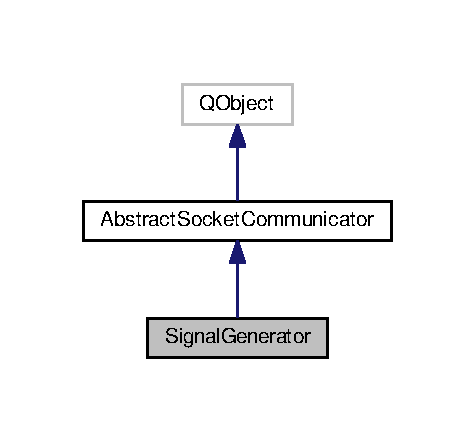
\includegraphics[width=228pt]{class_signal_generator__inherit__graph}
\end{center}
\end{figure}


Collaboration diagram for Signal\+Generator\+:\nopagebreak
\begin{figure}[H]
\begin{center}
\leavevmode
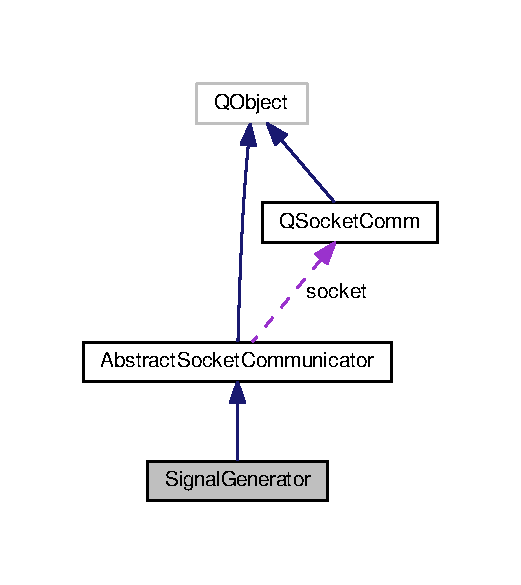
\includegraphics[width=250pt]{class_signal_generator__coll__graph}
\end{center}
\end{figure}
\subsection*{Public Member Functions}
\begin{DoxyCompactItemize}
\item 
{\bfseries Signal\+Generator} (std\+::string ip\+\_\+addr, uint port\+\_\+number, Q\+Object $\ast$parent=0)\hypertarget{class_signal_generator_a99405c3ab5e58876967fe4f7d34f84b3}{}\label{class_signal_generator_a99405c3ab5e58876967fe4f7d34f84b3}

\item 
\hyperlink{class_signal_generator}{Signal\+Generator} \& {\bfseries operator=} (const \hyperlink{class_signal_generator}{Signal\+Generator} \&)=delete\hypertarget{class_signal_generator_a4ee427365a76d62d3645f707cf1baf72}{}\label{class_signal_generator_a4ee427365a76d62d3645f707cf1baf72}

\item 
void {\bfseries R\+F\+On} ()\hypertarget{class_signal_generator_a55fbb51b7bd6b3cef69689eb8a63f0f9}{}\label{class_signal_generator_a55fbb51b7bd6b3cef69689eb8a63f0f9}

\item 
void {\bfseries R\+F\+Off} ()\hypertarget{class_signal_generator_a2f277765a848fe7640fae5b3d79c1714}{}\label{class_signal_generator_a2f277765a848fe7640fae5b3d79c1714}

\item 
void {\bfseries Set\+Frequency} (double freq\+\_\+\+M\+Hz)\hypertarget{class_signal_generator_a9ad69641992a00ef027682d5391df8e8}{}\label{class_signal_generator_a9ad69641992a00ef027682d5391df8e8}

\item 
void {\bfseries Set\+Power} (double power\+\_\+d\+Bm)\hypertarget{class_signal_generator_a319e0ca196dd341b1aab276626a729f3}{}\label{class_signal_generator_a319e0ca196dd341b1aab276626a729f3}

\end{DoxyCompactItemize}
\subsection*{Additional Inherited Members}


The documentation for this class was generated from the following files\+:\begin{DoxyCompactItemize}
\item 
/home/bephillips2/\+Qt-\/\+Projects/\+Electric\+\_\+\+Tiger\+\_\+\+D\+A\+Q/\+Socket\+Communicators/\+Signal\+Generator/signal\+\_\+generator.\+h\item 
/home/bephillips2/\+Qt-\/\+Projects/\+Electric\+\_\+\+Tiger\+\_\+\+D\+A\+Q/\+Socket\+Communicators/\+Signal\+Generator/signal\+\_\+generator.\+cpp\end{DoxyCompactItemize}

\hypertarget{class_socket_comm}{}\section{Socket\+Comm Class Reference}
\label{class_socket_comm}\index{Socket\+Comm@{Socket\+Comm}}
\subsection*{Public Member Functions}
\begin{DoxyCompactItemize}
\item 
{\bfseries Socket\+Comm} (std\+::string host\+\_\+name, uint port\+\_\+number)\hypertarget{class_socket_comm_a91848bdb00c5e2fa1d83bfabf2e83e23}{}\label{class_socket_comm_a91848bdb00c5e2fa1d83bfabf2e83e23}

\item 
void {\bfseries Send} (std\+::string command, std\+::string terminator=\char`\"{}\textbackslash{}n\char`\"{})\hypertarget{class_socket_comm_ad76f9593ad58c8899878d2b08ac61266}{}\label{class_socket_comm_ad76f9593ad58c8899878d2b08ac61266}

\item 
void {\bfseries Send\+Scl} (std\+::string command)\hypertarget{class_socket_comm_a9cda97b2727f4a47ef5f7d728737521b}{}\label{class_socket_comm_a9cda97b2727f4a47ef5f7d728737521b}

\item 
std\+::string {\bfseries Receive} ()\hypertarget{class_socket_comm_a854e742d1c9f998f7f0981fe3c77c84e}{}\label{class_socket_comm_a854e742d1c9f998f7f0981fe3c77c84e}

\item 
std\+::string {\bfseries Receive\+Safe} ()\hypertarget{class_socket_comm_a9c09a1bf47807b3465944a5555a61cec}{}\label{class_socket_comm_a9c09a1bf47807b3465944a5555a61cec}

\end{DoxyCompactItemize}


The documentation for this class was generated from the following files\+:\begin{DoxyCompactItemize}
\item 
/home/bephillips2/\+Qt-\/\+Projects/\+Electric\+\_\+\+Tiger\+\_\+\+D\+A\+Q/\+Socket\+Communicators/\+Socket\+Comm/socketcomm.\+h\item 
/home/bephillips2/\+Qt-\/\+Projects/\+Electric\+\_\+\+Tiger\+\_\+\+D\+A\+Q/\+Socket\+Communicators/\+Socket\+Comm/socketcomm.\+cpp\end{DoxyCompactItemize}

\hypertarget{class_spectrum_analyzer}{}\section{Spectrum\+Analyzer Class Reference}
\label{class_spectrum_analyzer}\index{Spectrum\+Analyzer@{Spectrum\+Analyzer}}


Inheritance diagram for Spectrum\+Analyzer\+:\nopagebreak
\begin{figure}[H]
\begin{center}
\leavevmode
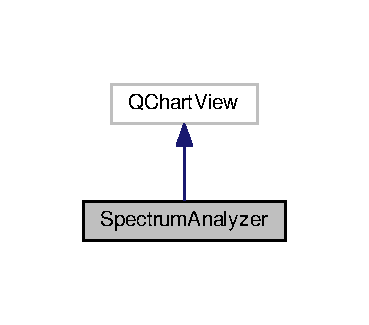
\includegraphics[width=177pt]{class_spectrum_analyzer__inherit__graph}
\end{center}
\end{figure}


Collaboration diagram for Spectrum\+Analyzer\+:\nopagebreak
\begin{figure}[H]
\begin{center}
\leavevmode
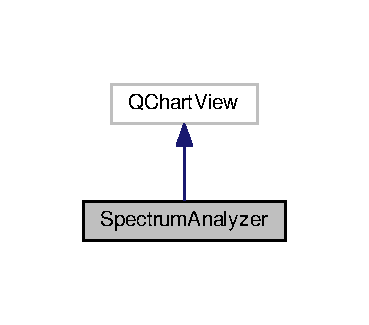
\includegraphics[width=177pt]{class_spectrum_analyzer__coll__graph}
\end{center}
\end{figure}
\subsection*{Public Slots}
\begin{DoxyCompactItemize}
\item 
void {\bfseries Update\+Signal} (std\+::vector$<$ float $>$ time\+\_\+series, uint sample\+\_\+rate)\hypertarget{class_spectrum_analyzer_aa1979b784bdb752d6f635c4cecb9a4b6}{}\label{class_spectrum_analyzer_aa1979b784bdb752d6f635c4cecb9a4b6}

\item 
void {\bfseries Set\+Frequency\+Min} (double min\+\_\+frequency)\hypertarget{class_spectrum_analyzer_a442e34f2e52a974bc33d614c4714a9e3}{}\label{class_spectrum_analyzer_a442e34f2e52a974bc33d614c4714a9e3}

\item 
void {\bfseries Set\+Power\+Min} (double min\+\_\+power)\hypertarget{class_spectrum_analyzer_aeb522d65cc87a8491f2480b3ec1cf133}{}\label{class_spectrum_analyzer_aeb522d65cc87a8491f2480b3ec1cf133}

\item 
void {\bfseries Set\+Frequency\+Max} (double max\+\_\+frequency)\hypertarget{class_spectrum_analyzer_ad1d9bf78ce633b097641ee092645daae}{}\label{class_spectrum_analyzer_ad1d9bf78ce633b097641ee092645daae}

\item 
void {\bfseries Set\+Power\+Max} (double max\+\_\+power)\hypertarget{class_spectrum_analyzer_adcaf09fb5f0449b6dd95b97e2469af47}{}\label{class_spectrum_analyzer_adcaf09fb5f0449b6dd95b97e2469af47}

\item 
void {\bfseries Change\+To\+Volts} ()\hypertarget{class_spectrum_analyzer_a7edc26864d46ebddd34257ff0d6bc8b7}{}\label{class_spectrum_analyzer_a7edc26864d46ebddd34257ff0d6bc8b7}

\item 
void {\bfseries Change\+Tod\+Bm} ()\hypertarget{class_spectrum_analyzer_af8f497cd56535515bc17319236fb0524}{}\label{class_spectrum_analyzer_af8f497cd56535515bc17319236fb0524}

\item 
void {\bfseries Auto\+Scale\+On} ()\hypertarget{class_spectrum_analyzer_a5370e5bdbd0ada33968251465658fd08}{}\label{class_spectrum_analyzer_a5370e5bdbd0ada33968251465658fd08}

\item 
void {\bfseries Auto\+Scale\+Off} ()\hypertarget{class_spectrum_analyzer_a033bdac1dd490537ab6ead20059b8c6e}{}\label{class_spectrum_analyzer_a033bdac1dd490537ab6ead20059b8c6e}

\end{DoxyCompactItemize}
\subsection*{Signals}
\begin{DoxyCompactItemize}
\item 
void {\bfseries Signal\+Changed} ()\hypertarget{class_spectrum_analyzer_afcbb7dc1848df0eb7d43160e489b8855}{}\label{class_spectrum_analyzer_afcbb7dc1848df0eb7d43160e489b8855}

\end{DoxyCompactItemize}
\subsection*{Public Member Functions}
\begin{DoxyCompactItemize}
\item 
{\bfseries Spectrum\+Analyzer} (Q\+Widget $\ast$parent=0)\hypertarget{class_spectrum_analyzer_aef258c587abbeb0b11cb765e5aeee636}{}\label{class_spectrum_analyzer_aef258c587abbeb0b11cb765e5aeee636}

\item 
void {\bfseries Plot\+Auto\+Scale} (const std\+::vector$<$ float $>$ \&y\+\_\+signal\+\_\+elements, float x\+\_\+frequency\+\_\+range)\hypertarget{class_spectrum_analyzer_a065ff36f268a12550ee3ca7fc0309e34}{}\label{class_spectrum_analyzer_a065ff36f268a12550ee3ca7fc0309e34}

\item 
void {\bfseries Plot} (const std\+::vector$<$ float $>$ \&y\+\_\+signal\+\_\+elements, float x\+\_\+frequency\+\_\+range)\hypertarget{class_spectrum_analyzer_a3fa614a77514275af0b0b82fbdd712a8}{}\label{class_spectrum_analyzer_a3fa614a77514275af0b0b82fbdd712a8}

\end{DoxyCompactItemize}


The documentation for this class was generated from the following files\+:\begin{DoxyCompactItemize}
\item 
/home/bephillips2/\+Qt-\/\+Projects/\+Electric\+\_\+\+Tiger\+\_\+\+D\+A\+Q/\+Panels/\+Spectrum\+Analyzer/spectrumanalyzer.\+h\item 
/home/bephillips2/\+Qt-\/\+Projects/\+Electric\+\_\+\+Tiger\+\_\+\+D\+A\+Q/\+Panels/\+Spectrum\+Analyzer/spectrumanalyzer.\+cpp\end{DoxyCompactItemize}

\hypertarget{class_stepper_motor}{}\section{Stepper\+Motor Class Reference}
\label{class_stepper_motor}\index{Stepper\+Motor@{Stepper\+Motor}}


Object to sends commands to an Applied Motion products stepper motor.  




{\ttfamily \#include $<$stepper\+\_\+motor.\+h$>$}



Inheritance diagram for Stepper\+Motor\+:\nopagebreak
\begin{figure}[H]
\begin{center}
\leavevmode
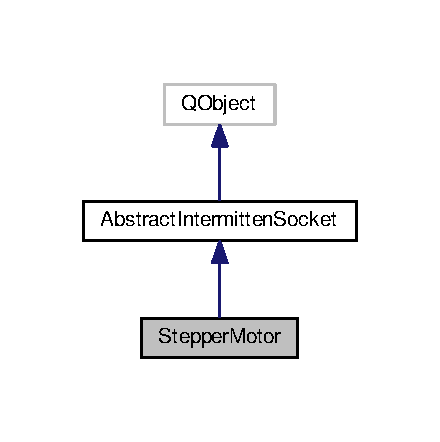
\includegraphics[width=211pt]{class_stepper_motor__inherit__graph}
\end{center}
\end{figure}


Collaboration diagram for Stepper\+Motor\+:\nopagebreak
\begin{figure}[H]
\begin{center}
\leavevmode
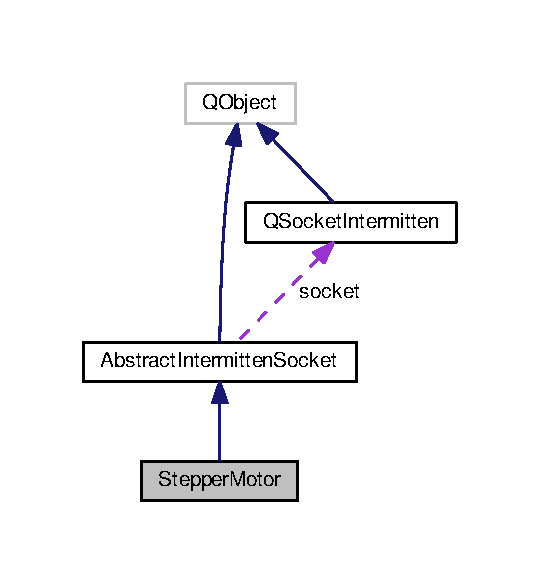
\includegraphics[width=259pt]{class_stepper_motor__coll__graph}
\end{center}
\end{figure}
\subsection*{Public Member Functions}
\begin{DoxyCompactItemize}
\item 
{\bfseries Stepper\+Motor} (std\+::string ip\+\_\+addr, uint port\+\_\+number, Q\+Object $\ast$parent=0)\hypertarget{class_stepper_motor_a6452f15d157117668e70de3e6b2b0b92}{}\label{class_stepper_motor_a6452f15d157117668e70de3e6b2b0b92}

\item 
\hyperlink{class_stepper_motor}{Stepper\+Motor} \& {\bfseries operator=} (const \hyperlink{class_stepper_motor}{Stepper\+Motor} \&)=delete\hypertarget{class_stepper_motor_aeeceb8eefbcffef0cb0c2b742ffe3603}{}\label{class_stepper_motor_aeeceb8eefbcffef0cb0c2b742ffe3603}

\item 
void {\bfseries Tune\+To\+Length} (double desired\+\_\+length, double current\+\_\+length)\hypertarget{class_stepper_motor_a5170955211342f0234e83897f552bec8}{}\label{class_stepper_motor_a5170955211342f0234e83897f552bec8}

\item 
void {\bfseries Tune\+Cavity} (double length\+\_\+of\+\_\+tune)\hypertarget{class_stepper_motor_a94ae4b10d58ea4dde277c05acf444bdf}{}\label{class_stepper_motor_a94ae4b10d58ea4dde277c05acf444bdf}

\item 
void {\bfseries Panic\+Reset\+Cavity} (uint iteration, double revs\+\_\+per\+\_\+iter)\hypertarget{class_stepper_motor_a260af15a346488150de82fa3801df94c}{}\label{class_stepper_motor_a260af15a346488150de82fa3801df94c}

\item 
void {\bfseries Tuning\+Loop} (double len\+\_\+of\+\_\+tune, double revs, uint iters)\hypertarget{class_stepper_motor_a6e140a11cb19bac6819978b5bb6d5a4d}{}\label{class_stepper_motor_a6e140a11cb19bac6819978b5bb6d5a4d}

\end{DoxyCompactItemize}
\subsection*{Additional Inherited Members}


\subsection{Detailed Description}
Object to sends commands to an Applied Motion products stepper motor. 

The documentation for this class was generated from the following files\+:\begin{DoxyCompactItemize}
\item 
/home/bephillips2/\+Qt-\/\+Projects/\+Electric\+\_\+\+Tiger\+\_\+\+D\+A\+Q/\+Socket\+Communicators/\+Stepper\+Motor/stepper\+\_\+motor.\+h\item 
/home/bephillips2/\+Qt-\/\+Projects/\+Electric\+\_\+\+Tiger\+\_\+\+D\+A\+Q/\+Socket\+Communicators/\+Stepper\+Motor/stepper\+\_\+motor.\+cpp\end{DoxyCompactItemize}

\hypertarget{class_switch}{}\section{Switch Class Reference}
\label{class_switch}\index{Switch@{Switch}}


Inheritance diagram for Switch\+:\nopagebreak
\begin{figure}[H]
\begin{center}
\leavevmode
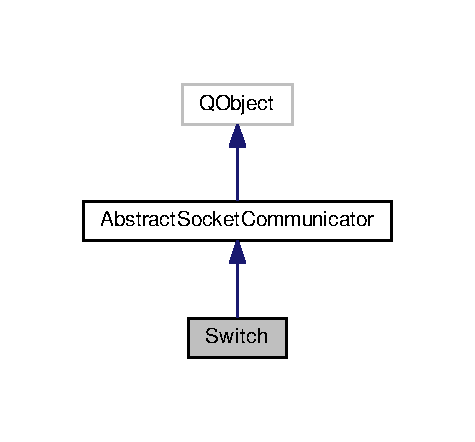
\includegraphics[width=228pt]{class_switch__inherit__graph}
\end{center}
\end{figure}


Collaboration diagram for Switch\+:\nopagebreak
\begin{figure}[H]
\begin{center}
\leavevmode
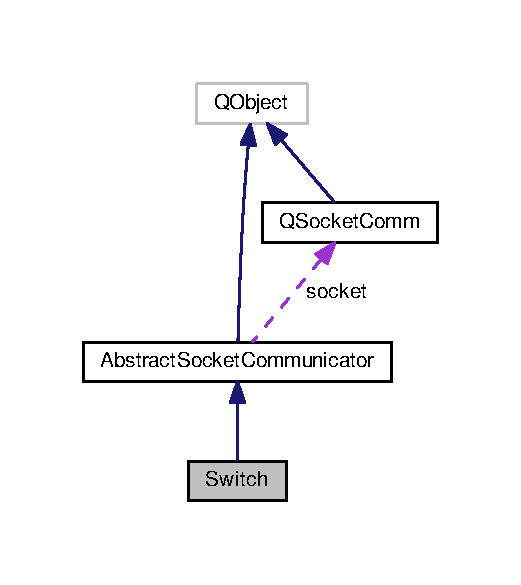
\includegraphics[width=250pt]{class_switch__coll__graph}
\end{center}
\end{figure}
\subsection*{Public Member Functions}
\begin{DoxyCompactItemize}
\item 
{\bfseries Switch} (std\+::string ip\+\_\+addr, uint port\+\_\+number, Q\+Object $\ast$parent=0)\hypertarget{class_switch_a65000fb5fb00f6833ec685175be47027}{}\label{class_switch_a65000fb5fb00f6833ec685175be47027}

\item 
\hyperlink{class_switch}{Switch} \& {\bfseries operator=} (const \hyperlink{class_switch}{Switch} \&)=delete\hypertarget{class_switch_a5d75382f2acb13883c3ef60d8b2aef7d}{}\label{class_switch_a5d75382f2acb13883c3ef60d8b2aef7d}

\item 
void {\bfseries Switch\+To\+Network\+Analyzer} ()\hypertarget{class_switch_a88b6be045896b8946be86202dc4c97e3}{}\label{class_switch_a88b6be045896b8946be86202dc4c97e3}

\item 
void {\bfseries Switch\+To\+Digitizer} ()\hypertarget{class_switch_a004bbaf7459b48549f87f7b26e9353ed}{}\label{class_switch_a004bbaf7459b48549f87f7b26e9353ed}

\item 
void {\bfseries Switch\+To\+Transmission} ()\hypertarget{class_switch_a9671dbed18c34b5e0e4c8961004d150e}{}\label{class_switch_a9671dbed18c34b5e0e4c8961004d150e}

\item 
void {\bfseries Switch\+To\+Reflection} ()\hypertarget{class_switch_abe4a4b4754fdb4979ddfa3a10fc9e127}{}\label{class_switch_abe4a4b4754fdb4979ddfa3a10fc9e127}

\end{DoxyCompactItemize}
\subsection*{Additional Inherited Members}


The documentation for this class was generated from the following files\+:\begin{DoxyCompactItemize}
\item 
/home/bephillips2/\+Qt-\/\+Projects/\+Electric\+\_\+\+Tiger\+\_\+\+D\+A\+Q/\+Socket\+Communicators/\+Switch/switch.\+h\item 
/home/bephillips2/\+Qt-\/\+Projects/\+Electric\+\_\+\+Tiger\+\_\+\+D\+A\+Q/\+Socket\+Communicators/\+Switch/switch.\+cpp\end{DoxyCompactItemize}

\hypertarget{struct_t_c_p_socket_param}{}\section{T\+C\+P\+Socket\+Param Struct Reference}
\label{struct_t_c_p_socket_param}\index{T\+C\+P\+Socket\+Param@{T\+C\+P\+Socket\+Param}}
\subsection*{Public Member Functions}
\begin{DoxyCompactItemize}
\item 
{\bfseries T\+C\+P\+Socket\+Param} (std\+::string name, std\+::string addr, uint port)\hypertarget{struct_t_c_p_socket_param_a5f8019ff9672a165db2c225cf86946cb}{}\label{struct_t_c_p_socket_param_a5f8019ff9672a165db2c225cf86946cb}

\item 
{\bfseries T\+C\+P\+Socket\+Param} (const std\+::string \&name, const std\+::string \&addr, uint port)\hypertarget{struct_t_c_p_socket_param_a30919df41998fdf63b706543c55d6bfa}{}\label{struct_t_c_p_socket_param_a30919df41998fdf63b706543c55d6bfa}

\item 
\hyperlink{struct_t_c_p_socket_param}{T\+C\+P\+Socket\+Param} \& {\bfseries operator=} (const \hyperlink{struct_t_c_p_socket_param}{T\+C\+P\+Socket\+Param} \&sock\+\_\+param)\hypertarget{struct_t_c_p_socket_param_a1440243b424ee42cf29c972b609b044a}{}\label{struct_t_c_p_socket_param_a1440243b424ee42cf29c972b609b044a}

\end{DoxyCompactItemize}
\subsection*{Public Attributes}
\begin{DoxyCompactItemize}
\item 
const std\+::string {\bfseries inst\+\_\+name}\hypertarget{struct_t_c_p_socket_param_adbcd0c094d7e3a8f8b083689ddccaff0}{}\label{struct_t_c_p_socket_param_adbcd0c094d7e3a8f8b083689ddccaff0}

\item 
const std\+::string {\bfseries ip\+\_\+addr}\hypertarget{struct_t_c_p_socket_param_a4dc4a074c147c36e0b281f7c25a96185}{}\label{struct_t_c_p_socket_param_a4dc4a074c147c36e0b281f7c25a96185}

\item 
const uint {\bfseries port\+\_\+addr}\hypertarget{struct_t_c_p_socket_param_a25103ad0fba22c679759538a8e2061b9}{}\label{struct_t_c_p_socket_param_a25103ad0fba22c679759538a8e2061b9}

\item 
std\+::string {\bfseries inst\+\_\+name}\hypertarget{struct_t_c_p_socket_param_ac6dd6cff76fe32d52214c39c8541201e}{}\label{struct_t_c_p_socket_param_ac6dd6cff76fe32d52214c39c8541201e}

\item 
std\+::string {\bfseries ip\+\_\+addr}\hypertarget{struct_t_c_p_socket_param_a4f424a058098e28b8a51c5d17b1fdc8a}{}\label{struct_t_c_p_socket_param_a4f424a058098e28b8a51c5d17b1fdc8a}

\item 
uint {\bfseries port\+\_\+addr}\hypertarget{struct_t_c_p_socket_param_a32da96a5f7f1aa3fe92db4454fba947c}{}\label{struct_t_c_p_socket_param_a32da96a5f7f1aa3fe92db4454fba947c}

\end{DoxyCompactItemize}
\subsection*{Friends}
\begin{DoxyCompactItemize}
\item 
std\+::ostream \& {\bfseries operator$<$$<$} (std\+::ostream \&stream, \hyperlink{struct_t_c_p_socket_param}{T\+C\+P\+Socket\+Param} \&param)\hypertarget{struct_t_c_p_socket_param_a2d9b78bcfdce6bdc7e301d7e819114c7}{}\label{struct_t_c_p_socket_param_a2d9b78bcfdce6bdc7e301d7e819114c7}

\item 
std\+::ostream \& {\bfseries operator$<$$<$} (std\+::ostream \&stream, \hyperlink{struct_t_c_p_socket_param}{T\+C\+P\+Socket\+Param} \&param)\hypertarget{struct_t_c_p_socket_param_a2d9b78bcfdce6bdc7e301d7e819114c7}{}\label{struct_t_c_p_socket_param_a2d9b78bcfdce6bdc7e301d7e819114c7}

\end{DoxyCompactItemize}


The documentation for this struct was generated from the following files\+:\begin{DoxyCompactItemize}
\item 
/home/bephillips2/\+Qt-\/\+Projects/\+Electric\+\_\+\+Tiger\+\_\+\+D\+A\+Q/\+Config\+Processor/configprocessor.\+h\item 
/home/bephillips2/\+Qt-\/\+Projects/\+Electric\+\_\+\+Tiger\+\_\+\+D\+A\+Q/\+Generics/generics.\+h\end{DoxyCompactItemize}

\hypertarget{class_test_config_processor}{}\section{Test\+Config\+Processor Class Reference}
\label{class_test_config_processor}\index{Test\+Config\+Processor@{Test\+Config\+Processor}}


The documentation for this class was generated from the following files\+:\begin{DoxyCompactItemize}
\item 
/home/bephillips2/\+Qt-\/\+Projects/\+Electric\+\_\+\+Tiger\+\_\+\+D\+A\+Q/\+Config\+Processor/testconfigprocessor.\+h\item 
/home/bephillips2/\+Qt-\/\+Projects/\+Electric\+\_\+\+Tiger\+\_\+\+D\+A\+Q/\+Config\+Processor/testconfigprocessor.\+cpp\end{DoxyCompactItemize}

\hypertarget{classetig_1_1test_1_1_test_instrument_view}{}\section{etig\+:\+:test\+:\+:Test\+Instrument\+View Class Reference}
\label{classetig_1_1test_1_1_test_instrument_view}\index{etig\+::test\+::\+Test\+Instrument\+View@{etig\+::test\+::\+Test\+Instrument\+View}}
\subsection*{Public Member Functions}
\begin{DoxyCompactItemize}
\item 
void {\bfseries Test} ()\hypertarget{classetig_1_1test_1_1_test_instrument_view_acca5fdef980dd4941b1d935de6bceac9}{}\label{classetig_1_1test_1_1_test_instrument_view_acca5fdef980dd4941b1d935de6bceac9}

\end{DoxyCompactItemize}


The documentation for this class was generated from the following files\+:\begin{DoxyCompactItemize}
\item 
/home/bephillips2/\+Qt-\/\+Projects/\+Electric\+\_\+\+Tiger\+\_\+\+D\+A\+Q/\+Panels/\+Instrument\+View/test\+\_\+instrumentview.\+h\item 
/home/bephillips2/\+Qt-\/\+Projects/\+Electric\+\_\+\+Tiger\+\_\+\+D\+A\+Q/\+Panels/\+Instrument\+View/test\+\_\+instrumentview.\+cpp\end{DoxyCompactItemize}

\hypertarget{classetig_1_1test_1_1_test_panels}{}\section{etig\+:\+:test\+:\+:Test\+Panels Class Reference}
\label{classetig_1_1test_1_1_test_panels}\index{etig\+::test\+::\+Test\+Panels@{etig\+::test\+::\+Test\+Panels}}
\subsection*{Public Member Functions}
\begin{DoxyCompactItemize}
\item 
void {\bfseries Test} ()\hypertarget{classetig_1_1test_1_1_test_panels_ae437513aa805be6ba2c046e3c83b862a}{}\label{classetig_1_1test_1_1_test_panels_ae437513aa805be6ba2c046e3c83b862a}

\end{DoxyCompactItemize}


The documentation for this class was generated from the following files\+:\begin{DoxyCompactItemize}
\item 
/home/bephillips2/\+Qt-\/\+Projects/\+Electric\+\_\+\+Tiger\+\_\+\+D\+A\+Q/\+Panels/testpanels.\+h\item 
/home/bephillips2/\+Qt-\/\+Projects/\+Electric\+\_\+\+Tiger\+\_\+\+D\+A\+Q/\+Panels/testpanels.\+cpp\end{DoxyCompactItemize}

\hypertarget{classetig_1_1test_1_1_test_spectrum_analyzer}{}\section{etig\+:\+:test\+:\+:Test\+Spectrum\+Analyzer Class Reference}
\label{classetig_1_1test_1_1_test_spectrum_analyzer}\index{etig\+::test\+::\+Test\+Spectrum\+Analyzer@{etig\+::test\+::\+Test\+Spectrum\+Analyzer}}
\subsection*{Public Member Functions}
\begin{DoxyCompactItemize}
\item 
void {\bfseries Test} ()\hypertarget{classetig_1_1test_1_1_test_spectrum_analyzer_ab09e54d9caf626da632d0bb52c223b1c}{}\label{classetig_1_1test_1_1_test_spectrum_analyzer_ab09e54d9caf626da632d0bb52c223b1c}

\end{DoxyCompactItemize}


The documentation for this class was generated from the following files\+:\begin{DoxyCompactItemize}
\item 
/home/bephillips2/\+Qt-\/\+Projects/\+Electric\+\_\+\+Tiger\+\_\+\+D\+A\+Q/\+Panels/\+Spectrum\+Analyzer/test\+\_\+spectrum\+\_\+analyzer.\+h\item 
/home/bephillips2/\+Qt-\/\+Projects/\+Electric\+\_\+\+Tiger\+\_\+\+D\+A\+Q/\+Panels/\+Spectrum\+Analyzer/test\+\_\+spectrum\+\_\+analyzer.\+cpp\end{DoxyCompactItemize}

\hypertarget{structetig_1_1test_1_1_volts_sqr_tod_bm}{}\section{etig\+:\+:test\+:\+:Volts\+Sqr\+Tod\+Bm Struct Reference}
\label{structetig_1_1test_1_1_volts_sqr_tod_bm}\index{etig\+::test\+::\+Volts\+Sqr\+Tod\+Bm@{etig\+::test\+::\+Volts\+Sqr\+Tod\+Bm}}
\subsection*{Public Member Functions}
\begin{DoxyCompactItemize}
\item 
void {\bfseries operator()} (\hyperlink{structdata__triple}{data\+\_\+triple}$<$ double $>$ \&data) const \hypertarget{structetig_1_1test_1_1_volts_sqr_tod_bm_acee890024218eb2188f7cdbd2a44b29b}{}\label{structetig_1_1test_1_1_volts_sqr_tod_bm_acee890024218eb2188f7cdbd2a44b29b}

\end{DoxyCompactItemize}


The documentation for this struct was generated from the following file\+:\begin{DoxyCompactItemize}
\item 
/home/bephillips2/\+Qt-\/\+Projects/\+Electric\+\_\+\+Tiger\+\_\+\+D\+A\+Q/\+Mode\+Characterization/test\+\_\+modecharacterization.\+h\end{DoxyCompactItemize}

%--- End generated contents ---

% Index
\backmatter
\newpage
\phantomsection
\clearemptydoublepage
\addcontentsline{toc}{chapter}{Index}
\printindex

\end{document}
